\section{The Prime Number Theorem and finding primes}

We'll need a way to create huge primes for RSA.

Of course you know Euclid's theorem that says
there are infinitely many primes.
So we don't have to worry about not finding them.
But just because there are infinitely many primes, it does not mean
they are everywhere!

Generally, we want to specify how large our primes should be.
This is specified by the bit length of the primes.
Given the length, one can generate a sequence of bit of that length.
Of course that number should be odd.
So the least significant bit is set to $1$.
Call this $n$.
One can than check if $n$ is a prime.
If $n$ is not prime, we try $n + 2$, etc.

Does this process take a long time?

Gauss was the first to realize that even though primes seem to appear
randomly on the real line,
\begin{center}
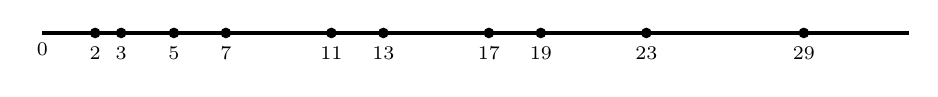
\begin{tikzpicture}
\draw[line width=0.04cm,black] (0,0) to  (11.0,0);

\fill[black] (0.67, 0.0) circle (0.06);
\draw[black] (0.67, 0.0) circle (0.06);
\node[anchor=north] at (0.67,-0.06)   {{\scriptsize $2$}};

\fill[black] (1.0, 0.0) circle (0.06);
\draw[black] (1.0, 0.0) circle (0.06);
\node[anchor=north] at (1.0,-0.06)   {{\scriptsize $3$}};

\fill[black] (1.67, 0.0) circle (0.06);
\draw[black] (1.67, 0.0) circle (0.06);
\node[anchor=north] at (1.67,-0.06)   {{\scriptsize $5$}};

\fill[black] (2.33, 0.0) circle (0.06);
\draw[black] (2.33, 0.0) circle (0.06);
\node[anchor=north] at (2.33,-0.06)   {{\scriptsize $7$}};

\fill[black] (3.67, 0.0) circle (0.06);
\draw[black] (3.67, 0.0) circle (0.06);
\node[anchor=north] at (3.67,-0.06)   {{\scriptsize $11$}};

\fill[black] (4.33, 0.0) circle (0.06);
\draw[black] (4.33, 0.0) circle (0.06);
\node[anchor=north] at (4.33,-0.06)   {{\scriptsize $13$}};

\fill[black] (5.67, 0.0) circle (0.06);
\draw[black] (5.67, 0.0) circle (0.06);
\node[anchor=north] at (5.67,-0.06)   {{\scriptsize $17$}};

\fill[black] (6.33, 0.0) circle (0.06);
\draw[black] (6.33, 0.0) circle (0.06);
\node[anchor=north] at (6.33,-0.06)   {{\scriptsize $19$}};

\fill[black] (7.67, 0.0) circle (0.06);
\draw[black] (7.67, 0.0) circle (0.06);
\node[anchor=north] at (7.67,-0.06)   {{\scriptsize $23$}};

\fill[black] (9.67, 0.0) circle (0.06);
\draw[black] (9.67, 0.0) circle (0.06);
\node[anchor=north] at (9.67,-0.06)   {{\scriptsize $29$}};

\node[anchor=north] at (0,0)   {{\scriptsize $0$}};
\end{tikzpicture}

\end{center}


the density of primes seems to follow some
law.
The density of primes can be defined this way.
Let $\pi(x)$ be the number of primes $\leq x$.
Then the density of primes up to $x$ is
\[
\frac{\pi(x)}{x}
\]
Here is the plot of $\pi(x)$ up to $x = 20$:

\begin{center}
\begin{tikzpicture}
\begin{axis}[width=5in, height=3in,
             xlabel={\mbox{}},
             xlabel style={name=xlabel}, 
             legend style={
                at={(xlabel.south)},
                yshift=-1ex,
                anchor=north,
                legend cell align=left,
                }
]
\addplot [black] coordinates {(0,0) (1,0) (2,0) (2,1) (3,1) (3,2) (4,2) (5,2) (5,3) (6,3) (7,3) (7,4) (8,4) (9,4) (10,4) (11,4) (11,5) (12,5) (13,5) (13,6) (14,6) (15,6) (16,6) (17,6) (17,7) (18,7) (19,7) (19,8)};

\legend{$\pi(x)$,
        $x/\ln x$}
\end{axis}
\end{tikzpicture}
\end{center}


When the plot is up to $x = 100$ one begin to see that the
rough and jagged graph begin to smooth out:

\begin{center}
\begin{tikzpicture}
\begin{axis}[width=5in, height=3in,
             xlabel={\mbox{}},
             xlabel style={name=xlabel}, 
             legend style={
                at={(xlabel.south)},
                yshift=-1ex,
                anchor=north,
                legend cell align=left,
                }
]
\addplot [black] coordinates {(0,0) (1,0) (2,0) (2,1) (3,1) (3,2) (4,2) (5,2) (5,3) (6,3) (7,3) (7,4) (8,4) (9,4) (10,4) (11,4) (11,5) (12,5) (13,5) (13,6) (14,6) (15,6) (16,6) (17,6) (17,7) (18,7) (19,7) (19,8) (20,8) (21,8) (22,8) (23,8) (23,9) (24,9) (25,9) (26,9) (27,9) (28,9) (29,9) (29,10) (30,10) (31,10) (31,11) (32,11) (33,11) (34,11) (35,11) (36,11) (37,11) (37,12) (38,12) (39,12) (40,12) (41,12) (41,13) (42,13) (43,13) (43,14) (44,14) (45,14) (46,14) (47,14) (47,15) (48,15) (49,15) (50,15) (51,15) (52,15) (53,15) (53,16) (54,16) (55,16) (56,16) (57,16) (58,16) (59,16) (59,17) (60,17) (61,17) (61,18) (62,18) (63,18) (64,18) (65,18) (66,18) (67,18) (67,19) (68,19) (69,19) (70,19) (71,19) (71,20) (72,20) (73,20) (73,21) (74,21) (75,21) (76,21) (77,21) (78,21) (79,21) (79,22) (80,22) (81,22) (82,22) (83,22) (83,23) (84,23) (85,23) (86,23) (87,23) (88,23) (89,23) (89,24) (90,24) (91,24) (92,24) (93,24) (94,24) (95,24) (96,24) (97,24) (97,25) (98,25) (99,25)};

\legend{$\pi(x)$,
        $x/\ln x$}
\end{axis}
\end{tikzpicture}
\end{center}



Through analyzing tables of primes, Gauss discovered that
$\pi(x)/x$ is \defone{asymptotically equivalent} to $1/\ln x$ ($\ln = \log_e$)
\[
\frac{\pi(x)}{x} \sim \frac{1}{\ln x}
\]
i.e.,
\[
\lim_{x \rightarrow \infty} \frac{\pi(x)/x}{1/\ln x} = 1
\]
Equivalently
\[
\pi(x) \sim \frac{x}{\ln x}
\]
Here a plot of $\pi(x)$ and $x/\ln x$ up to $x = 10^5$:

\begin{center}
\begin{tikzpicture}
\begin{axis}[width=5in, height=3in,
             xlabel={\mbox{}},
             xlabel style={name=xlabel}, 
             legend style={
                at={(xlabel.south)},
                yshift=-1ex,
                anchor=north,
                legend cell align=left,
                }
]
\addplot [black] coordinates {(0,0) (7,3) (14,6) (22,8) (30,10) (38,12) (46,14) (54,16) (62,18) (71,19) (79,21) (87,23) (96,24) (103,27) (111,29) (120,30) (129,31) (137,33) (146,34) (154,36) (163,37) (171,39) (179,41) (188,42) (196,44) (204,46) (213,47) (223,47) (230,50) (239,51) (247,53) (256,54) (264,56) (272,58) (281,59) (289,61) (298,62) (307,63) (315,65) (324,66) (333,67) (342,68) (350,70) (359,71) (367,73) (376,74) (384,76) (393,77) (401,79) (410,80) (419,81) (428,82) (436,84) (444,86) (453,87) (461,89) (469,91) (479,91) (487,93) (496,94) (504,96) (513,97) (522,98) (531,99) (541,99) (549,101) (558,102) (567,103) (575,105) (584,106) (593,107) (601,109) (609,111) (617,113) (626,114) (635,115) (643,117) (652,118) (660,120) (669,121) (677,123) (686,124) (695,125) (704,126) (713,127) (722,128) (731,129) (739,131) (748,132) (757,133) (765,135) (773,137) (783,137) (792,138) (801,139) (810,140) (819,141) (827,143) (835,145) (844,146) (853,147) (861,149) (870,150) (879,151) (887,153) (896,154) (906,154) (914,156) (923,157) (932,158) (941,159) (949,161) (958,162) (967,163) (976,164) (984,166) (993,167) (1002,168) (1011,169) (1019,171) (1028,172) (1036,174) (1045,175) (1053,177) (1062,178) (1070,180) (1080,180) (1089,181) (1097,183) (1105,185) (1114,186) (1123,187) (1131,189) (1141,189) (1151,189) (1159,191) (1168,192) (1177,193) (1186,194) (1194,196) (1203,197) (1213,197) (1221,199) (1229,201) (1237,203) (1247,203) (1256,204) (1265,205) (1275,205) (1283,207) (1291,209) (1299,211) (1307,213) (1316,214) (1324,216) (1333,217) (1343,217) (1353,217) (1362,218) (1371,219) (1380,220) (1389,221) (1399,221) (1408,222) (1417,223) (1426,224) (1433,227) (1442,228) (1451,229) (1459,231) (1468,232) (1477,233) (1485,235) (1493,237) (1501,239) (1511,239) (1520,240) (1529,241) (1538,242) (1547,243) (1555,245) (1564,246) (1572,248) (1581,249) (1590,250) (1599,251) (1607,253) (1615,255) (1623,257) (1632,258) (1641,259) (1651,259) (1660,260) (1668,262) (1677,263) (1687,263) (1696,264) (1704,266) (1713,267) (1722,268) (1731,269) (1740,270) (1748,272) (1757,273) (1766,274) (1776,274) (1784,276) (1792,278) (1801,279) (1811,279) (1820,280) (1829,281) (1838,282) (1847,283) (1857,283) (1866,284) (1873,287) (1881,289) (1890,290) (1900,290) (1908,292) (1917,293) (1927,293) (1935,295) (1945,295) (1953,297) (1963,297) (1973,297) (1981,299) (1990,300) (1998,302) (2006,304) (2015,305) (2024,306) (2032,308) (2041,309) (2051,309) (2060,310) (2069,311) (2078,312) (2086,314) (2094,316) (2103,317) (2112,318) (2121,319) (2130,320) (2138,322) (2146,324) (2155,325) (2164,326) (2174,326) (2183,327) (2193,327) (2203,327) (2211,329) (2220,330) (2229,331) (2238,332) (2246,334) (2255,335) (2265,335) (2273,337) (2281,339) (2290,340) (2298,342) (2308,342) (2316,344) (2326,344) (2335,345) (2343,347) (2351,349) (2360,350) (2370,350) (2378,352) (2386,354) (2394,356) (2403,357) (2412,358) (2421,359) (2430,360) (2439,361) (2447,363) (2457,363) (2466,364) (2474,366) (2483,367) (2493,367) (2503,367) (2512,368) (2521,369) (2531,369) (2539,371) (2548,372) (2556,374) (2565,375) (2575,375) (2584,376) (2593,377) (2602,378) (2611,379) (2620,380) (2629,381) (2638,382) (2647,383) (2657,383) (2664,386) (2673,387) (2682,388) (2689,391) (2698,392) (2707,393) (2714,396) (2723,397) (2731,399) (2741,399) (2749,401) (2758,402) (2767,403) (2777,403) (2786,404) (2794,406) (2802,408) (2811,409) (2820,410) (2830,410) (2838,412) (2847,413) (2856,414) (2864,416) (2874,416) (2883,417) (2892,418) (2901,419) (2909,421) (2918,422) (2927,423) (2937,423) (2946,424) (2955,425) (2963,427) (2971,429) (2981,429) (2991,429) (3000,430) (3009,431) (3018,432) (3026,434) (3036,434) (3044,436) (3053,437) (3062,438) (3071,439) (3080,440) (3089,441) (3098,442) (3108,442) (3117,443) (3125,445) (3135,445) (3144,446) (3154,446) (3163,447) (3171,449) (3181,449) (3189,451) (3198,452) (3207,453) (3216,454) (3224,456) (3233,457) (3243,457) (3252,458) (3259,461) (3269,461) (3278,462) (3288,462) (3298,462) (3306,464) (3314,466) (3323,467) (3331,469) (3340,470) (3348,472) (3358,472) (3366,474) (3374,476) (3384,476) (3392,478) (3402,478) (3411,479) (3420,480) (3430,480) (3439,481) (3449,481) (3457,483) (3465,485) (3473,487) (3483,487) (3492,488) (3501,489) (3511,489) (3519,491) (3528,492) (3536,494) (3544,496) (3553,497) (3561,499) (3571,499) (3580,500) (3588,502) (3597,503) (3607,503) (3615,505) (3623,507) (3632,508) (3641,509) (3650,510) (3659,511) (3669,511) (3677,513) (3686,514) (3695,515) (3703,517) (3712,518) (3721,519) (3730,520) (3739,521) (3748,522) (3758,522) (3767,523) (3775,525) (3784,526) (3793,527) (3802,528) (3811,529) (3821,529) (3829,531) (3838,532) (3847,533) (3855,535) (3864,536) (3874,536) (3882,538) (3891,539) (3901,539) (3910,540) (3918,542) (3926,544) (3934,546) (3943,547) (3952,548) (3962,548) (3971,549) (3981,549) (3990,550) (4000,550) (4007,553) (4016,554) (4024,556) (4033,557) (4043,557) (4051,559) (4060,560) (4070,560) (4079,561) (4088,562) (4096,564) (4105,565) (4114,566) (4124,566) (4132,568) (4140,570) (4150,570) (4158,572) (4167,573) (4177,573) (4186,574) (4196,574) (4205,575) (4214,576) (4222,578) (4231,579) (4240,580) (4248,582) (4257,583) (4265,585) (4273,587) (4283,587) (4291,589) (4300,590) (4310,590) (4320,590) (4329,591) (4338,592) (4347,593) (4356,594) (4364,596) (4373,597) (4383,597) (4392,598) (4401,599) (4410,600) (4420,600) (4428,602) (4438,602) (4447,603) (4455,605) (4463,607) (4473,607) (4482,608) (4491,609) (4500,610) (4509,611) (4517,613) (4525,615) (4535,615) (4545,615) (4553,617) (4562,618) (4571,619) (4581,619) (4590,620) (4598,622) (4607,623) (4617,623) (4626,624) (4636,624) (4643,627) (4651,629) (4660,630) (4669,631) (4678,632) (4687,633) (4696,634) (4705,635) (4715,635) (4723,637) (4732,638) (4741,639) (4751,639) (4759,641) (4769,641) (4779,641) (4787,643) (4795,645) (4803,647) (4813,647) (4821,649) (4831,649) (4840,650) (4850,650) (4860,650) (4869,651) (4877,653) (4887,653) (4896,654) (4905,655) (4914,656) (4923,657) (4932,658) (4940,660) (4949,661) (4957,663) (4967,663) (4974,666) (4984,666) (4993,667) (5001,669) (5009,671) (5018,672) (5026,674) (5036,674) (5045,675) (5054,676) (5063,677) (5073,677) (5081,679) (5090,680) (5099,681) (5107,683) (5116,684) (5125,685) (5135,685) (5145,685) (5153,687) (5163,687) (5171,689) (5180,690) (5189,691) (5198,692) (5208,692) (5217,693) (5227,693) (5234,696) (5243,697) (5253,697) (5262,698) (5272,698) (5280,700) (5289,701) (5298,702) (5307,703) (5316,704) (5325,705) (5334,706) (5344,706) (5352,708) (5362,708) (5372,708) (5381,709) (5390,710) (5399,711) (5407,713) (5416,714) (5424,716) (5433,717) (5441,719) (5449,721) (5459,721) (5469,721) (5477,723) (5485,725) (5495,725) (5503,727) (5512,728) (5521,729) (5529,731) (5538,732) (5548,732) (5557,733) (5566,734) (5574,736) (5583,737) (5592,738) (5602,738) (5612,738) (5622,738) (5631,739) (5640,740) (5648,742) (5656,744) (5664,746) (5673,747) (5683,747) (5691,749) (5700,750) (5709,751) (5717,753) (5727,753) (5737,753) (5744,756) (5753,757) (5763,757) (5773,757) (5782,758) (5791,759) (5800,760) (5808,762) (5817,763) (5826,764) (5835,765) (5843,767) (5851,769) (5860,770) (5868,772) (5877,773) (5885,775) (5895,775) (5903,777) (5913,777) (5923,777) (5931,779) (5940,780) (5950,780) (5959,781) (5969,781) (5979,781) (5987,783) (5997,783) (6007,783) (6015,785) (6025,785) (6034,786) (6043,787) (6051,789) (6060,790) (6069,791) (6078,792) (6087,793) (6095,795) (6104,796) (6113,797) (6122,798) (6131,799) (6140,800) (6149,801) (6158,802) (6167,803) (6176,804) (6186,804) (6196,804) (6203,807) (6212,808) (6221,809) (6229,811) (6239,811) (6248,812) (6257,813) (6266,814) (6274,816) (6283,817) (6292,818) (6301,819) (6310,820) (6318,822) (6327,823) (6336,824) (6344,826) (6353,827) (6361,829) (6370,830) (6379,831) (6388,832) (6397,833) (6406,834) (6416,834) (6425,835) (6434,836) (6444,836) (6452,838) (6462,838) (6471,839) (6480,840) (6489,841) (6498,842) (6508,842) (6518,842) (6527,843) (6536,844) (6546,844) (6553,847) (6563,847) (6571,849) (6579,851) (6588,852) (6598,852) (6607,853) (6616,854) (6625,855) (6635,855) (6644,856) (6653,857) (6661,859) (6671,859) (6679,861) (6689,861) (6697,863) (6705,865) (6714,866) (6723,867) (6733,867) (6741,869) (6751,869) (6761,869) (6769,871) (6779,871) (6787,873) (6795,875) (6804,876) (6814,876) (6823,877) (6831,879) (6840,880) (6849,881) (6858,882) (6867,883) (6875,885) (6884,886) (6894,886) (6903,887) (6911,889) (6920,890) (6930,890) (6940,890) (6949,891) (6958,892) (6966,894) (6974,896) (6983,897) (6991,899) (7000,900) (7009,901) (7018,902) (7027,903) (7036,904) (7044,906) (7054,906) (7063,907) (7072,908) (7081,909) (7091,909) (7101,909) (7109,911) (7119,911) (7127,913) (7136,914) (7146,914) (7155,915) (7164,916) (7174,916) (7183,917) (7192,918) (7201,919) (7210,920) (7218,922) (7227,923) (7236,924) (7244,926) (7253,927) (7262,928) (7272,928) (7282,928) (7291,929) (7300,930) (7309,931) (7318,932) (7327,933) (7335,935) (7345,935) (7353,937) (7363,937) (7372,938) (7382,938) (7392,938) (7401,939) (7411,939) (7419,941) (7429,941) (7438,942) (7448,942) (7457,943) (7465,945) (7475,945) (7483,947) (7491,949) (7500,950) (7509,951) (7518,952) (7527,953) (7536,954) (7544,956) (7552,958) (7561,959) (7570,960) (7578,962) (7587,963) (7595,965) (7604,966) (7613,967) (7622,968) (7632,968) (7641,969) (7649,971) (7659,971) (7669,971) (7677,973) (7686,974) (7694,976) (7703,977) (7712,978) (7721,979) (7729,981) (7739,981) (7748,982) (7757,983) (7765,985) (7775,985) (7785,985) (7793,987) (7803,987) (7813,987) (7822,988) (7830,990) (7840,990) (7849,991) (7858,992) (7867,993) (7876,994) (7883,997) (7893,997) (7902,998) (7911,999) (7920,1000) (7929,1001) (7937,1003) (7947,1003) (7955,1005) (7964,1006) (7974,1006) (7984,1006) (7993,1007) (8003,1007) (8011,1009) (8020,1010) (8030,1010) (8039,1011) (8049,1011) (8058,1012) (8067,1013) (8076,1014) (8085,1015) (8093,1017) (8101,1019) (8111,1019) (8119,1021) (8128,1022) (8138,1022) (8147,1023) (8157,1023) (8166,1024) (8174,1026) (8183,1027) (8192,1028) (8202,1028) (8211,1029) (8220,1030) (8229,1031) (8237,1033) (8245,1035) (8255,1035) (8264,1036) (8273,1037) (8282,1038) (8291,1039) (8298,1042) (8308,1042) (8317,1043) (8326,1044) (8335,1045) (8345,1045) (8354,1046) (8363,1047) (8372,1048) (8381,1049) (8389,1051) (8399,1051) (8409,1051) (8419,1051) (8427,1053) (8435,1055) (8444,1056) (8453,1057) (8462,1058) (8471,1059) (8481,1059) (8491,1059) (8501,1059) (8510,1060) (8519,1061) (8527,1063) (8537,1063) (8544,1066) (8554,1066) (8563,1067) (8573,1067) (8581,1069) (8591,1069) (8599,1071) (8609,1071) (8618,1072) (8627,1073) (8635,1075) (8644,1076) (8653,1077) (8663,1077) (8671,1079) (8680,1080) (8689,1081) (8697,1083) (8706,1084) (8714,1086) (8723,1087) (8732,1088) (8741,1089) (8749,1091) (8758,1092) (8767,1093) (8777,1093) (8785,1095) (8795,1095) (8804,1096) (8813,1097) (8821,1099) (8831,1099) (8839,1101) (8848,1102) (8857,1103) (8865,1105) (8874,1106) (8884,1106) (8893,1107) (8902,1108) (8912,1108) (8922,1108) (8930,1110) (8939,1111) (8948,1112) (8957,1113) (8966,1114) (8974,1116) (8984,1116) (8994,1116) (9002,1118) (9011,1119) (9019,1121) (9029,1121) (9038,1122) (9046,1124) (9055,1125) (9064,1126) (9073,1127) (9083,1127) (9092,1128) (9102,1128) (9110,1130) (9120,1130) (9129,1131) (9137,1133) (9147,1133) (9156,1134) (9164,1136) (9173,1137) (9182,1138) (9191,1139) (9200,1140) (9209,1141) (9218,1142) (9227,1143) (9236,1144) (9244,1146) (9254,1146) (9263,1147) (9273,1147) (9281,1149) (9290,1150) (9299,1151) (9309,1151) (9318,1152) (9326,1154) (9336,1154) (9343,1157) (9352,1158) (9362,1158) (9371,1159) (9380,1160) (9390,1160) (9398,1162) (9407,1163) (9416,1164) (9424,1166) (9433,1167) (9440,1170) (9450,1170) (9460,1170) (9467,1173) (9476,1174) (9485,1175) (9494,1176) (9503,1177) (9512,1178) (9521,1179) (9531,1179) (9539,1181) (9548,1182) (9557,1183) (9567,1183) (9577,1183) (9587,1183) (9596,1184) (9605,1185) (9614,1186) (9623,1187) (9631,1189) (9640,1190) (9649,1191) (9658,1192) (9667,1193) (9677,1193) (9685,1195) (9694,1196) (9703,1197) (9713,1197) (9721,1199) (9731,1199) (9739,1201) (9748,1202) (9757,1203) (9767,1203) (9775,1205) (9784,1206) (9792,1208) (9802,1208) (9811,1209) (9819,1211) (9829,1211) (9837,1213) (9846,1214) (9855,1215) (9863,1217) (9872,1218) (9882,1218) (9890,1220) (9900,1220) (9908,1222) (9918,1222) (9927,1223) (9935,1225) (9944,1226) (9953,1227) (9963,1227) (9972,1228) (9981,1229) (9991,1229) (10001,1229) (10009,1231) (10019,1231) (10029,1231) (10038,1232) (10047,1233) (10057,1233) (10066,1234) (10074,1236) (10083,1237) (10092,1238) (10100,1240) (10109,1241) (10118,1242) (10128,1242) (10137,1243) (10145,1245) (10154,1246) (10163,1247) (10171,1249) (10180,1250) (10189,1251) (10198,1252) (10208,1252) (10217,1253) (10226,1254) (10236,1254) (10245,1255) (10253,1257) (10262,1258) (10271,1259) (10279,1261) (10289,1261) (10298,1262) (10306,1264) (10315,1265) (10324,1266) (10333,1267) (10341,1269) (10350,1270) (10359,1271) (10369,1271) (10378,1272) (10388,1272) (10397,1273) (10406,1274) (10416,1274) (10426,1274) (10433,1277) (10443,1277) (10453,1277) (10460,1280) (10469,1281) (10478,1282) (10487,1283) (10497,1283) (10505,1285) (10514,1286) (10524,1286) (10532,1288) (10542,1288) (10552,1288) (10561,1289) (10570,1290) (10580,1290) (10589,1291) (10598,1292) (10607,1293) (10615,1295) (10625,1295) (10633,1297) (10642,1298) (10651,1299) (10660,1300) (10668,1302) (10678,1302) (10687,1303) (10696,1304) (10706,1304) (10714,1306) (10723,1307) (10732,1308) (10740,1310) (10750,1310) (10759,1311) (10769,1311) (10778,1312) (10787,1313) (10796,1314) (10805,1315) (10815,1315) (10825,1315) (10834,1316) (10843,1317) (10852,1318) (10860,1320) (10868,1322) (10878,1322) (10887,1323) (10895,1325) (10904,1326) (10913,1327) (10923,1327) (10933,1327) (10941,1329) (10950,1330) (10959,1331) (10969,1331) (10978,1332) (10987,1333) (10995,1335) (11004,1336) (11014,1336) (11024,1336) (11033,1337) (11043,1337) (11052,1338) (11060,1340) (11069,1341) (11078,1342) (11087,1343) (11095,1345) (11105,1345) (11114,1346) (11122,1348) (11131,1349) (11141,1349) (11150,1350) (11159,1351) (11168,1352) (11176,1354) (11185,1355) (11195,1355) (11204,1356) (11213,1357) (11223,1357) (11233,1357) (11242,1358) (11251,1359) (11259,1361) (11268,1362) (11277,1363) (11286,1364) (11295,1365) (11304,1366) (11313,1367) (11321,1369) (11330,1370) (11340,1370) (11350,1370) (11358,1372) (11368,1372) (11377,1373) (11386,1374) (11395,1375) (11404,1376) (11413,1377) (11423,1377) (11432,1378) (11441,1379) (11449,1381) (11459,1381) (11468,1382) (11477,1383) (11486,1384) (11494,1386) (11503,1387) (11512,1388) (11521,1389) (11530,1390) (11540,1390) (11549,1391) (11558,1392) (11568,1392) (11578,1392) (11587,1393) (11595,1395) (11604,1396) (11614,1396) (11622,1398) (11632,1398) (11641,1399) (11651,1399) (11660,1400) (11670,1400) (11679,1401) (11688,1402) (11697,1403) (11705,1405) (11715,1405) (11723,1407) (11732,1408) (11742,1408) (11751,1409) (11761,1409) (11771,1409) (11779,1411) (11788,1412) (11797,1413) (11806,1414) (11814,1416) (11823,1417) (11831,1419) (11839,1421) (11849,1421) (11859,1421) (11867,1423) (11877,1423) (11887,1423) (11896,1424) (11904,1426) (11913,1427) (11923,1427) (11931,1429) (11939,1431) (11948,1432) (11957,1433) (11966,1434) (11974,1436) (11983,1437) (11992,1438) (12002,1438) (12011,1439) (12020,1440) (12030,1440) (12039,1441) (12047,1443) (12056,1444) (12066,1444) (12074,1446) (12084,1446) (12094,1446) (12102,1448) (12110,1450) (12119,1451) (12128,1452) (12138,1452) (12147,1453) (12156,1454) (12163,1457) (12173,1457) (12183,1457) (12193,1457) (12202,1458) (12211,1459) (12220,1460) (12229,1461) (12239,1461) (12247,1463) (12255,1465) (12264,1466) (12273,1467) (12281,1469) (12290,1470) (12300,1470) (12309,1471) (12319,1471) (12328,1472) (12337,1473) (12346,1474) (12355,1475) (12365,1475) (12374,1476) (12382,1478) (12391,1479) (12401,1479) (12409,1481) (12418,1482) (12427,1483) (12436,1484) (12445,1485) (12454,1486) (12463,1487) (12473,1487) (12481,1489) (12490,1490) (12498,1492) (12507,1493) (12516,1494) (12525,1495) (12534,1496) (12542,1498) (12551,1499) (12560,1500) (12569,1501) (12578,1502) (12587,1503) (12596,1504) (12605,1505) (12613,1507) (12622,1508) (12632,1508) (12641,1509) (12649,1511) (12658,1512) (12667,1513) (12676,1514) (12686,1514) (12695,1515) (12703,1517) (12713,1517) (12721,1519) (12731,1519) (12740,1520) (12749,1521) (12758,1522) (12767,1523) (12777,1523) (12786,1524) (12795,1525) (12804,1526) (12813,1527) (12822,1528) (12830,1530) (12840,1530) (12849,1531) (12858,1532) (12868,1532) (12878,1532) (12888,1532) (12896,1534) (12905,1535) (12913,1537) (12921,1539) (12930,1540) (12940,1540) (12949,1541) (12958,1542) (12967,1543) (12975,1545) (12983,1547) (12993,1547) (13002,1548) (13009,1551) (13019,1551) (13029,1551) (13037,1553) (13046,1554) (13055,1555) (13064,1556) (13074,1556) (13084,1556) (13093,1557) (13102,1558) (13110,1560) (13120,1560) (13128,1562) (13138,1562) (13147,1563) (13156,1564) (13164,1566) (13173,1567) (13182,1568) (13190,1570) (13200,1570) (13210,1570) (13219,1571) (13228,1572) (13237,1573) (13246,1574) (13255,1575) (13264,1576) (13273,1577) (13283,1577) (13292,1578) (13301,1579) (13310,1580) (13319,1581) (13328,1582) (13337,1583) (13345,1585) (13355,1585) (13365,1585) (13374,1586) (13383,1587) (13393,1587) (13401,1589) (13411,1589) (13419,1591) (13428,1592) (13438,1592) (13447,1593) (13456,1594) (13464,1596) (13473,1597) (13482,1598) (13491,1599) (13500,1600) (13510,1600) (13519,1601) (13528,1602) (13537,1603) (13547,1603) (13556,1604) (13566,1604) (13575,1605) (13584,1606) (13593,1607) (13602,1608) (13612,1608) (13620,1610) (13629,1611) (13638,1612) (13648,1612) (13657,1613) (13667,1613) (13676,1614) (13684,1616) (13692,1618) (13700,1620) (13709,1621) (13718,1622) (13726,1624) (13735,1625) (13745,1625) (13754,1626) (13762,1628) (13771,1629) (13781,1629) (13789,1631) (13799,1631) (13807,1633) (13817,1633) (13827,1633) (13835,1635) (13844,1636) (13854,1636) (13863,1637) (13873,1637) (13880,1640) (13889,1641) (13899,1641) (13907,1643) (13915,1645) (13924,1646) (13933,1647) (13942,1648) (13952,1648) (13962,1648) (13970,1650) (13980,1650) (13990,1650) (13999,1651) (14008,1652) (14016,1654) (14026,1654) (14034,1656) (14044,1656) (14053,1657) (14062,1658) (14071,1659) (14081,1659) (14088,1662) (14098,1662) (14107,1663) (14117,1663) (14127,1663) (14137,1663) (14146,1664) (14154,1666) (14163,1667) (14173,1667) (14181,1669) (14191,1669) (14200,1670) (14209,1671) (14219,1671) (14228,1672) (14238,1672) (14247,1673) (14255,1675) (14265,1675) (14275,1675) (14284,1676) (14293,1677) (14303,1677) (14312,1678) (14321,1679) (14329,1681) (14339,1681) (14347,1683) (14357,1683) (14367,1683) (14376,1684) (14386,1684) (14394,1686) (14403,1687) (14411,1689) (14420,1690) (14429,1691) (14437,1693) (14447,1693) (14455,1695) (14464,1696) (14474,1696) (14483,1697) (14492,1698) (14502,1698) (14511,1699) (14520,1700) (14530,1700) (14538,1702) (14547,1703) (14555,1705) (14563,1707) (14572,1708) (14582,1708) (14591,1709) (14600,1710) (14610,1710) (14620,1710) (14628,1712) (14636,1714) (14645,1715) (14654,1716) (14663,1717) (14672,1718) (14682,1718) (14691,1719) (14700,1720) (14710,1720) (14718,1722) (14727,1723) (14736,1724) (14744,1726) (14753,1727) (14761,1729) (14770,1730) (14779,1731) (14787,1733) (14797,1733) (14806,1734) (14815,1735) (14824,1736) (14832,1738) (14842,1738) (14851,1739) (14860,1740) (14869,1741) (14878,1742) (14887,1743) (14895,1745) (14904,1746) (14914,1746) (14923,1747) (14932,1748) (14941,1749) (14950,1750) (14958,1752) (14968,1752) (14977,1753) (14986,1754) (14996,1754) (15006,1754) (15015,1755) (15024,1756) (15033,1757) (15043,1757) (15053,1757) (15061,1759) (15071,1759) (15079,1761) (15088,1762) (15097,1763) (15106,1764) (15115,1765) (15124,1766) (15133,1767) (15141,1769) (15150,1770) (15160,1770) (15169,1771) (15178,1772) (15187,1773) (15196,1774) (15205,1775) (15215,1775) (15224,1776) (15233,1777) (15241,1779) (15251,1779) (15260,1780) (15269,1781) (15277,1783) (15286,1784) (15294,1786) (15303,1787) (15312,1788) (15320,1790) (15329,1791) (15338,1792) (15348,1792) (15357,1793) (15365,1795) (15374,1796) (15383,1797) (15391,1799) (15401,1799) (15410,1800) (15419,1801) (15428,1802) (15438,1802) (15446,1804) (15455,1805) (15464,1806) (15473,1807) (15482,1808) (15492,1808) (15500,1810) (15510,1810) (15519,1811) (15528,1812) (15538,1812) (15547,1813) (15556,1814) (15565,1815) (15574,1816) (15583,1817) (15592,1818) (15601,1819) (15610,1820) (15619,1821) (15629,1821) (15638,1822) (15646,1824) (15654,1826) (15663,1827) (15671,1829) (15680,1830) (15689,1831) (15699,1831) (15709,1831) (15719,1831) (15728,1832) (15736,1834) (15744,1836) (15753,1837) (15762,1838) (15771,1839) (15780,1840) (15789,1841) (15797,1843) (15806,1844) (15815,1845) (15823,1847) (15833,1847) (15843,1847) (15853,1847) (15862,1848) (15872,1848) (15881,1849) (15889,1851) (15898,1852) (15907,1853) (15915,1855) (15923,1857) (15933,1857) (15942,1858) (15952,1858) (15961,1859) (15971,1859) (15979,1861) (15989,1861) (15998,1862) (16007,1863) (16016,1864) (16026,1864) (16035,1865) (16045,1865) (16055,1865) (16063,1867) (16070,1870) (16079,1871) (16088,1872) (16097,1873) (16105,1875) (16114,1876) (16124,1876) (16133,1877) (16141,1879) (16151,1879) (16161,1879) (16171,1879) (16181,1879) (16189,1881) (16197,1883) (16207,1883) (16217,1883) (16225,1885) (16233,1887) (16243,1887) (16252,1888) (16261,1889) (16270,1890) (16279,1891) (16289,1891) (16299,1891) (16308,1892) (16318,1892) (16327,1893) (16336,1894) (16345,1895) (16354,1896) (16363,1897) (16371,1899) (16381,1899) (16390,1900) (16400,1900) (16410,1900) (16418,1902) (16427,1903) (16435,1905) (16445,1905) (16453,1907) (16462,1908) (16472,1908) (16481,1909) (16489,1911) (16498,1912) (16508,1912) (16518,1912) (16527,1913) (16536,1914) (16546,1914) (16554,1916) (16563,1917) (16572,1918) (16581,1919) (16591,1919) (16601,1919) (16609,1921) (16619,1921) (16628,1922) (16636,1924) (16646,1924) (16654,1926) (16662,1928) (16672,1928) (16681,1929) (16691,1929) (16699,1931) (16707,1933) (16717,1933) (16727,1933) (16736,1934) (16745,1935) (16754,1936) (16763,1937) (16772,1938) (16782,1938) (16791,1939) (16801,1939) (16811,1939) (16820,1940) (16829,1941) (16837,1943) (16846,1944) (16856,1944) (16866,1944) (16875,1945) (16883,1947) (16892,1948) (16901,1949) (16910,1950) (16920,1950) (16928,1952) (16937,1953) (16945,1955) (16955,1955) (16964,1956) (16974,1956) (16982,1958) (16991,1959) (17000,1960) (17010,1960) (17019,1961) (17027,1963) (17035,1965) (17044,1966) (17053,1967) (17062,1968) (17072,1968) (17081,1969) (17091,1969) (17099,1971) (17108,1972) (17117,1973) (17126,1974) (17136,1974) (17145,1975) (17155,1975) (17164,1976) (17173,1977) (17183,1977) (17191,1979) (17200,1980) (17208,1982) (17217,1983) (17227,1983) (17236,1984) (17245,1985) (17255,1985) (17264,1986) (17274,1986) (17284,1986) (17293,1987) (17301,1989) (17311,1989) (17320,1990) (17328,1992) (17337,1993) (17346,1994) (17355,1995) (17364,1996) (17374,1996) (17383,1997) (17390,2000) (17399,2001) (17408,2002) (17417,2003) (17426,2004) (17435,2005) (17444,2006) (17453,2007) (17463,2007) (17471,2009) (17480,2010) (17489,2011) (17497,2013) (17506,2014) (17515,2015) (17524,2016) (17534,2016) (17543,2017) (17552,2018) (17562,2018) (17571,2019) (17579,2021) (17588,2022) (17597,2023) (17606,2024) (17615,2025) (17624,2026) (17633,2027) (17643,2027) (17653,2027) (17661,2029) (17670,2030) (17680,2030) (17688,2032) (17698,2032) (17707,2033) (17716,2034) (17726,2034) (17735,2035) (17744,2036) (17752,2038) (17761,2039) (17771,2039) (17781,2039) (17789,2041) (17798,2042) (17807,2043) (17817,2043) (17827,2043) (17836,2044) (17844,2046) (17853,2047) (17863,2047) (17872,2048) (17881,2049) (17891,2049) (17900,2050) (17909,2051) (17917,2053) (17925,2055) (17934,2056) (17943,2057) (17953,2057) (17961,2059) (17971,2059) (17979,2061) (17987,2063) (17996,2064) (18006,2064) (18015,2065) (18025,2065) (18035,2065) (18043,2067) (18051,2069) (18060,2070) (18069,2071) (18078,2072) (18088,2072) (18097,2073) (18106,2074) (18116,2074) (18124,2076) (18132,2078) (18141,2079) (18149,2081) (18159,2081) (18169,2081) (18178,2082) (18187,2083) (18196,2084) (18205,2085) (18214,2086) (18223,2087) (18231,2089) (18240,2090) (18250,2090) (18257,2093) (18267,2093) (18276,2094) (18286,2094) (18294,2096) (18303,2097) (18311,2099) (18320,2100) (18329,2101) (18339,2101) (18348,2102) (18357,2103) (18367,2103) (18375,2105) (18384,2106) (18394,2106) (18402,2108) (18412,2108) (18421,2109) (18430,2110) (18439,2111) (18447,2113) (18456,2114) (18464,2116) (18474,2116) (18483,2117) (18493,2117) (18502,2118) (18511,2119) (18520,2120) (18528,2122) (18538,2122) (18546,2124) (18555,2125) (18565,2125) (18575,2125) (18584,2126) (18593,2127) (18602,2128) (18612,2128) (18621,2129) (18631,2129) (18640,2130) (18650,2130) (18660,2130) (18669,2131) (18678,2132) (18687,2133) (18696,2134) (18705,2135) (18714,2136) (18723,2137) (18732,2138) (18742,2138) (18750,2140) (18759,2141) (18769,2141) (18778,2142) (18787,2143) (18796,2144) (18804,2146) (18814,2146) (18824,2146) (18834,2146) (18843,2147) (18853,2147) (18862,2148) (18871,2149) (18881,2149) (18891,2149) (18900,2150) (18910,2150) (18917,2153) (18926,2154) (18936,2154) (18946,2154) (18955,2155) (18964,2156) (18973,2157) (18982,2158) (18992,2158) (19001,2159) (19010,2160) (19019,2161) (19029,2161) (19037,2163) (19047,2163) (19056,2164) (19066,2164) (19074,2166) (19082,2168) (19091,2169) (19101,2169) (19111,2169) (19121,2169) (19130,2170) (19139,2171) (19148,2172) (19157,2173) (19166,2174) (19176,2174) (19184,2176) (19194,2176) (19204,2176) (19212,2178) (19220,2180) (19230,2180) (19238,2182) (19248,2182) (19257,2183) (19266,2184) (19274,2186) (19284,2186) (19293,2187) (19302,2188) (19311,2189) (19320,2190) (19330,2190) (19339,2191) (19349,2191) (19359,2191) (19369,2191) (19378,2192) (19386,2194) (19394,2196) (19403,2197) (19413,2197) (19421,2199) (19429,2201) (19437,2203) (19446,2204) (19455,2205) (19463,2207) (19471,2209) (19480,2210) (19489,2211) (19498,2212) (19507,2213) (19516,2214) (19526,2214) (19535,2215) (19543,2217) (19553,2217) (19561,2219) (19571,2219) (19579,2221) (19588,2222) (19597,2223) (19606,2224) (19615,2225) (19625,2225) (19635,2225) (19645,2225) (19655,2225) (19664,2226) (19674,2226) (19683,2227) (19692,2228) (19700,2230) (19709,2231) (19718,2232) (19727,2233) (19737,2233) (19746,2234) (19754,2236) (19763,2237) (19772,2238) (19781,2239) (19791,2239) (19800,2240) (19809,2241) (19818,2242) (19827,2243) (19837,2243) (19845,2245) (19854,2246) (19863,2247) (19872,2248) (19882,2248) (19891,2249) (19900,2250) (19910,2250) (19919,2251) (19927,2253) (19937,2253) (19946,2254) (19955,2255) (19963,2257) (19973,2257) (19981,2259) (19991,2259) (19998,2262) (20008,2262) (20017,2263) (20025,2265) (20034,2266) (20044,2266) (20052,2268) (20062,2268) (20071,2269) (20080,2270) (20089,2271) (20099,2271) (20107,2273) (20116,2274) (20124,2276) (20133,2277) (20143,2277) (20150,2280) (20160,2280) (20169,2281) (20177,2283) (20186,2284) (20196,2284) (20205,2285) (20215,2285) (20224,2286) (20233,2287) (20242,2288) (20251,2289) (20261,2289) (20269,2291) (20279,2291) (20288,2292) (20297,2293) (20307,2293) (20317,2293) (20326,2294) (20334,2296) (20343,2297) (20352,2298) (20359,2301) (20369,2301) (20378,2302) (20388,2302) (20396,2304) (20405,2305) (20413,2307) (20423,2307) (20432,2308) (20441,2309) (20450,2310) (20460,2310) (20470,2310) (20479,2311) (20487,2313) (20497,2313) (20507,2313) (20515,2315) (20524,2316) (20533,2317) (20543,2317) (20551,2319) (20560,2320) (20569,2321) (20579,2321) (20589,2321) (20598,2322) (20607,2323) (20616,2324) (20626,2324) (20635,2325) (20643,2327) (20653,2327) (20663,2327) (20672,2328) (20681,2329) (20691,2329) (20700,2330) (20709,2331) (20718,2332) (20727,2333) (20736,2334) (20745,2335) (20753,2337) (20761,2339) (20771,2339) (20779,2341) (20789,2341) (20798,2342) (20807,2343) (20816,2344) (20826,2344) (20836,2344) (20846,2344) (20855,2345) (20864,2346) (20873,2347) (20882,2348) (20891,2349) (20899,2351) (20908,2352) (20918,2352) (20927,2353) (20936,2354) (20945,2355) (20954,2356) (20963,2357) (20972,2358) (20981,2359) (20990,2360) (21000,2360) (21009,2361) (21017,2363) (21024,2366) (21033,2367) (21043,2367) (21053,2367) (21061,2369) (21070,2370) (21080,2370) (21089,2371) (21099,2371) (21107,2373) (21117,2373) (21126,2374) (21136,2374) (21144,2376) (21153,2377) (21162,2378) (21170,2380) (21179,2381) (21188,2382) (21196,2384) (21206,2384) (21215,2385) (21224,2386) (21233,2387) (21243,2387) (21252,2388) (21262,2388) (21271,2389) (21280,2390) (21289,2391) (21299,2391) (21309,2391) (21317,2393) (21325,2395) (21335,2395) (21344,2396) (21353,2397) (21363,2397) (21373,2397) (21381,2399) (21390,2400) (21398,2402) (21407,2403) (21416,2404) (21425,2405) (21434,2406) (21444,2406) (21454,2406) (21464,2406) (21473,2407) (21482,2408) (21491,2409) (21499,2411) (21507,2413) (21517,2413) (21524,2416) (21533,2417) (21543,2417) (21553,2417) (21561,2419) (21569,2421) (21578,2422) (21587,2423) (21596,2424) (21604,2426) (21613,2427) (21621,2429) (21631,2429) (21641,2429) (21649,2431) (21659,2431) (21668,2432) (21677,2433) (21686,2434) (21696,2434) (21705,2435) (21714,2436) (21724,2436) (21733,2437) (21741,2439) (21751,2439) (21759,2441) (21768,2442) (21777,2443) (21787,2443) (21796,2444) (21804,2446) (21814,2446) (21822,2448) (21832,2448) (21841,2449) (21850,2450) (21859,2451) (21867,2453) (21876,2454) (21885,2455) (21894,2456) (21904,2456) (21913,2457) (21923,2457) (21932,2458) (21941,2459) (21950,2460) (21960,2460) (21969,2461) (21978,2462) (21988,2462) (21997,2463) (22005,2465) (22014,2466) (22024,2466) (22032,2468) (22040,2470) (22050,2470) (22059,2471) (22067,2473) (22076,2474) (22085,2475) (22093,2477) (22103,2477) (22111,2479) (22121,2479) (22129,2481) (22138,2482) (22147,2483) (22156,2484) (22164,2486) (22173,2487) (22183,2487) (22192,2488) (22201,2489) (22211,2489) (22221,2489) (22230,2490) (22240,2490) (22249,2491) (22259,2491) (22268,2492) (22276,2494) (22283,2497) (22292,2498) (22302,2498) (22310,2500) (22320,2500) (22330,2500) (22340,2500) (22349,2501) (22358,2502) (22367,2503) (22376,2504) (22385,2505) (22394,2506) (22403,2507) (22412,2508) (22422,2508) (22432,2508) (22441,2509) (22449,2511) (22458,2512) (22468,2512) (22477,2513) (22485,2515) (22495,2515) (22504,2516) (22513,2517) (22523,2517) (22532,2518) (22541,2519) (22549,2521) (22559,2521) (22568,2522) (22576,2524) (22586,2524) (22596,2524) (22606,2524) (22615,2525) (22623,2527) (22633,2527) (22641,2529) (22650,2530) (22659,2531) (22669,2531) (22678,2532) (22687,2533) (22696,2534) (22704,2536) (22713,2537) (22721,2539) (22730,2540) (22739,2541) (22748,2542) (22757,2543) (22767,2543) (22776,2544) (22784,2546) (22793,2547) (22803,2547) (22811,2549) (22820,2550) (22830,2550) (22840,2550) (22850,2550) (22859,2551) (22867,2553) (22876,2554) (22885,2555) (22895,2555) (22904,2556) (22913,2557) (22922,2558) (22932,2558) (22941,2559) (22950,2560) (22960,2560) (22968,2562) (22977,2563) (22987,2563) (22996,2564) (23005,2565) (23014,2566) (23022,2568) (23030,2570) (23039,2571) (23048,2572) (23057,2573) (23064,2576) (23073,2577) (23082,2578) (23091,2579) (23100,2580) (23110,2580) (23119,2581) (23129,2581) (23138,2582) (23147,2583) (23157,2583) (23166,2584) (23174,2586) (23184,2586) (23193,2587) (23201,2589) (23209,2591) (23219,2591) (23228,2592) (23238,2592) (23248,2592) (23257,2593) (23267,2593) (23276,2594) (23285,2595) (23293,2597) (23302,2598) (23311,2599) (23321,2599) (23329,2601) (23338,2602) (23347,2603) (23357,2603) (23366,2604) (23374,2606) (23384,2606) (23394,2606) (23403,2607) (23413,2607) (23422,2608) (23431,2609) (23441,2609) (23450,2610) (23459,2611) (23469,2611) (23478,2612) (23488,2612) (23497,2613) (23507,2613) (23516,2614) (23526,2614) (23535,2615) (23543,2617) (23552,2618) (23561,2619) (23568,2622) (23578,2622) (23587,2623) (23596,2624) (23604,2626) (23613,2627) (23623,2627) (23630,2630) (23639,2631) (23649,2631) (23659,2631) (23668,2632) (23676,2634) (23685,2635) (23693,2637) (23703,2637) (23713,2637) (23722,2638) (23732,2638) (23741,2639) (23749,2641) (23758,2642) (23767,2643) (23775,2645) (23785,2645) (23794,2646) (23803,2647) (23813,2647) (23821,2649) (23830,2650) (23838,2652) (23848,2652) (23857,2653) (23867,2653) (23875,2655) (23884,2656) (23893,2657) (23901,2659) (23910,2660) (23918,2662) (23928,2662) (23937,2663) (23947,2663) (23957,2663) (23966,2664) (23975,2665) (23983,2667) (23993,2667) (24001,2669) (24010,2670) (24019,2671) (24028,2672) (24037,2673) (24046,2674) (24055,2675) (24064,2676) (24073,2677) (24082,2678) (24091,2679) (24099,2681) (24107,2683) (24115,2685) (24124,2686) (24133,2687) (24142,2688) (24151,2689) (24161,2689) (24170,2690) (24179,2691) (24188,2692) (24197,2693) (24206,2694) (24216,2694) (24225,2695) (24234,2696) (24243,2697) (24251,2699) (24261,2699) (24271,2699) (24281,2699) (24290,2700) (24300,2700) (24310,2700) (24319,2701) (24329,2701) (24337,2703) (24347,2703) (24357,2703) (24366,2704) (24374,2706) (24383,2707) (24392,2708) (24402,2708) (24411,2709) (24419,2711) (24428,2712) (24438,2712) (24446,2714) (24456,2714) (24466,2714) (24474,2716) (24483,2717) (24493,2717) (24502,2718) (24511,2719) (24520,2720) (24529,2721) (24538,2722) (24547,2723) (24556,2724) (24566,2724) (24575,2725) (24585,2725) (24594,2726) (24604,2726) (24613,2727) (24623,2727) (24631,2729) (24641,2729) (24651,2729) (24660,2730) (24670,2730) (24678,2732) (24687,2733) (24696,2734) (24705,2735) (24714,2736) (24724,2736) (24733,2737) (24743,2737) (24752,2738) (24762,2738) (24770,2740) (24780,2740) (24789,2741) (24798,2742) (24807,2743) (24816,2744) (24825,2745) (24835,2745) (24844,2746) (24852,2748) (24861,2749) (24871,2749) (24880,2750) (24889,2751) (24899,2751) (24908,2752) (24917,2753) (24925,2755) (24935,2755) (24944,2756) (24953,2757) (24963,2757) (24971,2759) (24979,2761) (24989,2761) (24998,2762) (25008,2762) (25017,2763) (25027,2763) (25035,2765) (25044,2766) (25054,2766) (25063,2767) (25073,2767) (25082,2768) (25091,2769) (25100,2770) (25110,2770) (25118,2772) (25127,2773) (25136,2774) (25146,2774) (25154,2776) (25163,2777) (25171,2779) (25181,2779) (25189,2781) (25199,2781) (25209,2781) (25219,2781) (25228,2782) (25237,2783) (25245,2785) (25253,2787) (25262,2788) (25272,2788) (25282,2788) (25292,2788) (25301,2789) (25309,2791) (25318,2792) (25327,2793) (25337,2793) (25345,2795) (25354,2796) (25363,2797) (25372,2798) (25381,2799) (25391,2799) (25400,2800) (25409,2801) (25418,2802) (25427,2803) (25437,2803) (25446,2804) (25454,2806) (25463,2807) (25471,2809) (25480,2810) (25490,2810) (25500,2810) (25510,2810) (25520,2810) (25529,2811) (25538,2812) (25547,2813) (25557,2813) (25566,2814) (25576,2814) (25583,2817) (25592,2818) (25601,2819) (25609,2821) (25619,2821) (25628,2822) (25637,2823) (25645,2825) (25655,2825) (25664,2826) (25673,2827) (25681,2829) (25691,2829) (25700,2830) (25709,2831) (25718,2832) (25728,2832) (25737,2833) (25746,2834) (25755,2835) (25763,2837) (25772,2838) (25782,2838) (25792,2838) (25800,2840) (25809,2841) (25819,2841) (25828,2842) (25838,2842) (25847,2843) (25855,2845) (25865,2845) (25873,2847) (25883,2847) (25892,2848) (25902,2848) (25911,2849) (25919,2851) (25929,2851) (25937,2853) (25945,2855) (25954,2856) (25964,2856) (25973,2857) (25982,2858) (25992,2858) (26000,2860) (26009,2861) (26018,2862) (26027,2863) (26036,2864) (26045,2865) (26054,2866) (26064,2866) (26074,2866) (26083,2867) (26093,2867) (26102,2868) (26111,2869) (26119,2871) (26128,2872) (26138,2872) (26147,2873) (26156,2874) (26165,2875) (26174,2876) (26183,2877) (26191,2879) (26201,2879) (26209,2881) (26219,2881) (26228,2882) (26237,2883) (26247,2883) (26255,2885) (26263,2887) (26272,2888) (26282,2888) (26292,2888) (26300,2890) (26309,2891) (26318,2892) (26327,2893) (26337,2893) (26346,2894) (26355,2895) (26364,2896) (26373,2897) (26383,2897) (26392,2898) (26400,2900) (26409,2901) (26418,2902) (26427,2903) (26436,2904) (26445,2905) (26454,2906) (26463,2907) (26473,2907) (26482,2908) (26491,2909) (26500,2910) (26509,2911) (26518,2912) (26528,2912) (26538,2912) (26547,2913) (26557,2913) (26565,2915) (26574,2916) (26584,2916) (26593,2917) (26602,2918) (26612,2918) (26622,2918) (26631,2919) (26640,2920) (26648,2922) (26658,2922) (26668,2922) (26677,2923) (26685,2925) (26693,2927) (26701,2929) (26711,2929) (26718,2932) (26727,2933) (26735,2935) (26744,2936) (26754,2936) (26763,2937) (26773,2937) (26782,2938) (26791,2939) (26801,2939) (26810,2940) (26819,2941) (26828,2942) (26837,2943) (26846,2944) (26855,2945) (26863,2947) (26873,2947) (26881,2949) (26891,2949) (26899,2951) (26908,2952) (26918,2952) (26927,2953) (26936,2954) (26946,2954) (26953,2957) (26962,2958) (26972,2958) (26981,2959) (26990,2960) (26999,2961) (27009,2961) (27017,2963) (27027,2963) (27036,2964) (27045,2965) (27055,2965) (27063,2967) (27072,2968) (27080,2970) (27090,2970) (27099,2971) (27107,2973) (27116,2974) (27126,2974) (27135,2975) (27144,2976) (27154,2976) (27164,2976) (27174,2976) (27183,2977) (27192,2978) (27201,2979) (27211,2979) (27220,2980) (27230,2980) (27239,2981) (27248,2982) (27257,2983) (27266,2984) (27275,2985) (27283,2987) (27292,2988) (27301,2989) (27311,2989) (27321,2989) (27330,2990) (27339,2991) (27349,2991) (27359,2991) (27367,2993) (27377,2993) (27387,2993) (27397,2993) (27406,2994) (27414,2996) (27424,2996) (27432,2998) (27441,2999) (27450,3000) (27459,3001) (27469,3001) (27479,3001) (27487,3003) (27496,3004) (27506,3004) (27515,3005) (27525,3005) (27533,3007) (27541,3009) (27551,3009) (27560,3010) (27570,3010) (27580,3010) (27588,3012) (27598,3012) (27608,3012) (27617,3013) (27626,3014) (27635,3015) (27645,3015) (27653,3017) (27663,3017) (27673,3017) (27682,3018) (27691,3019) (27699,3021) (27708,3022) (27718,3022) (27728,3022) (27737,3023) (27744,3026) (27752,3028) (27762,3028) (27770,3030) (27779,3031) (27788,3032) (27796,3034) (27804,3036) (27813,3037) (27822,3038) (27830,3040) (27840,3040) (27849,3041) (27858,3042) (27868,3042) (27878,3042) (27887,3043) (27896,3044) (27905,3045) (27915,3045) (27923,3047) (27933,3047) (27942,3048) (27950,3050) (27959,3051) (27967,3053) (27977,3053) (27986,3054) (27996,3054) (28004,3056) (28014,3056) (28023,3057) (28031,3059) (28041,3059) (28051,3059) (28059,3061) (28069,3061) (28078,3062) (28087,3063) (28096,3064) (28104,3066) (28112,3068) (28122,3068) (28131,3069) (28141,3069) (28151,3069) (28160,3070) (28169,3071) (28179,3071) (28187,3073) (28197,3073) (28206,3074) (28215,3075) (28224,3076) (28233,3077) (28243,3077) (28253,3077) (28263,3077) (28273,3077) (28281,3079) (28289,3081) (28298,3082) (28307,3083) (28316,3084) (28325,3085) (28335,3085) (28345,3085) (28353,3087) (28363,3087) (28373,3087) (28383,3087) (28392,3088) (28401,3089) (28409,3091) (28418,3092) (28428,3092) (28436,3094) (28445,3095) (28454,3096) (28463,3097) (28473,3097) (28482,3098) (28492,3098) (28500,3100) (28510,3100) (28518,3102) (28528,3102) (28537,3103) (28546,3104) (28554,3106) (28563,3107) (28572,3108) (28580,3110) (28590,3110) (28598,3112) (28607,3113) (28616,3114) (28624,3116) (28632,3118) (28642,3118) (28650,3120) (28659,3121) (28667,3123) (28676,3124) (28686,3124) (28695,3125) (28703,3127) (28712,3128) (28722,3128) (28730,3130) (28740,3130) (28750,3130) (28758,3132) (28767,3133) (28776,3134) (28786,3134) (28794,3136) (28804,3136) (28813,3137) (28821,3139) (28831,3139) (28840,3140) (28849,3141) (28859,3141) (28867,3143) (28876,3144) (28885,3145) (28895,3145) (28904,3146) (28913,3147) (28922,3148) (28931,3149) (28940,3150) (28949,3151) (28959,3151) (28968,3152) (28978,3152) (28987,3153) (28997,3153) (29007,3153) (29016,3154) (29023,3157) (29032,3158) (29041,3159) (29051,3159) (29060,3160) (29069,3161) (29078,3162) (29088,3162) (29098,3162) (29107,3163) (29117,3163) (29126,3164) (29134,3166) (29143,3167) (29152,3168) (29161,3169) (29170,3170) (29179,3171) (29188,3172) (29197,3173) (29206,3174) (29214,3176) (29223,3177) (29232,3178) (29242,3178) (29251,3179) (29260,3180) (29269,3181) (29279,3181) (29288,3182) (29297,3183) (29306,3184) (29315,3185) (29325,3185) (29333,3187) (29342,3188) (29351,3189) (29361,3189) (29370,3190) (29380,3190) (29388,3192) (29397,3193) (29405,3195) (29414,3196) (29423,3197) (29432,3198) (29441,3199) (29450,3200) (29459,3201) (29469,3201) (29478,3202) (29487,3203) (29497,3203) (29506,3204) (29516,3204) (29526,3204) (29534,3206) (29543,3207) (29553,3207) (29563,3207) (29571,3209) (29580,3210) (29588,3212) (29598,3212) (29607,3213) (29616,3214) (29626,3214) (29634,3216) (29643,3217) (29653,3217) (29663,3217) (29671,3219) (29680,3220) (29689,3221) (29699,3221) (29709,3221) (29718,3222) (29727,3223) (29737,3223) (29746,3224) (29755,3225) (29763,3227) (29773,3227) (29783,3227) (29792,3228) (29802,3228) (29811,3229) (29820,3230) (29830,3230) (29838,3232) (29848,3232) (29857,3233) (29866,3234) (29874,3236) (29882,3238) (29892,3238) (29902,3238) (29912,3238) (29921,3239) (29929,3241) (29939,3241) (29948,3242) (29958,3242) (29967,3243) (29977,3243) (29986,3244) (29995,3245) (30005,3245) (30013,3247) (30023,3247) (30032,3248) (30042,3248) (30051,3249) (30060,3250) (30070,3250) (30079,3251) (30089,3251) (30097,3253) (30105,3255) (30113,3257) (30122,3258) (30132,3258) (30139,3261) (30149,3261) (30159,3261) (30168,3262) (30177,3263) (30186,3264) (30195,3265) (30203,3267) (30212,3268) (30222,3268) (30231,3269) (30241,3269) (30250,3270) (30259,3271) (30268,3272) (30276,3274) (30286,3274) (30295,3275) (30305,3275) (30313,3277) (30322,3278) (30331,3279) (30341,3279) (30349,3281) (30359,3281) (30368,3282) (30378,3282) (30388,3282) (30396,3284) (30405,3285) (30415,3285) (30425,3285) (30433,3287) (30443,3287) (30452,3288) (30462,3288) (30470,3290) (30480,3290) (30490,3290) (30497,3293) (30507,3293) (30516,3294) (30525,3295) (30534,3296) (30543,3297) (30553,3297) (30560,3300) (30570,3300) (30579,3301) (30589,3301) (30598,3302) (30608,3302) (30618,3302) (30628,3302) (30637,3303) (30645,3305) (30654,3306) (30663,3307) (30672,3308) (30681,3309) (30690,3310) (30699,3311) (30707,3313) (30716,3314) (30726,3314) (30735,3315) (30745,3315) (30755,3315) (30763,3317) (30773,3317) (30781,3319) (30791,3319) (30801,3319) (30809,3321) (30818,3322) (30828,3322) (30837,3323) (30845,3325) (30853,3327) (30862,3328) (30871,3329) (30880,3330) (30889,3331) (30898,3332) (30908,3332) (30917,3333) (30927,3333) (30936,3334) (30944,3336) (30953,3337) (30963,3337) (30972,3338) (30981,3339) (30990,3340) (31000,3340) (31010,3340) (31019,3341) (31028,3342) (31037,3343) (31046,3344) (31055,3345) (31064,3346) (31073,3347) (31081,3349) (31091,3349) (31100,3350) (31110,3350) (31120,3350) (31128,3352) (31138,3352) (31147,3353) (31154,3356) (31163,3357) (31173,3357) (31181,3359) (31189,3361) (31198,3362) (31208,3362) (31218,3362) (31226,3364) (31235,3365) (31244,3366) (31252,3368) (31260,3370) (31269,3371) (31277,3373) (31287,3373) (31297,3373) (31307,3373) (31316,3374) (31324,3376) (31333,3377) (31341,3379) (31351,3379) (31360,3380) (31370,3380) (31379,3381) (31388,3382) (31396,3384) (31405,3385) (31415,3385) (31425,3385) (31435,3385) (31445,3385) (31455,3385) (31465,3385) (31474,3386) (31482,3388) (31491,3389) (31501,3389) (31511,3389) (31518,3392) (31528,3392) (31537,3393) (31545,3395) (31554,3396) (31564,3396) (31573,3397) (31582,3398) (31591,3399) (31601,3399) (31609,3401) (31619,3401) (31628,3402) (31638,3402) (31647,3403) (31656,3404) (31664,3406) (31673,3407) (31683,3407) (31692,3408) (31701,3409) (31711,3409) (31721,3409) (31728,3412) (31737,3413) (31746,3414) (31755,3415) (31765,3415) (31773,3417) (31783,3417) (31793,3417) (31801,3419) (31811,3419) (31820,3420) (31830,3420) (31840,3420) (31849,3421) (31858,3422) (31867,3423) (31876,3424) (31885,3425) (31894,3426) (31904,3426) (31913,3427) (31923,3427) (31933,3427) (31943,3427) (31953,3427) (31962,3428) (31971,3429) (31980,3430) (31989,3431) (31998,3432) (32007,3433) (32016,3434) (32026,3434) (32034,3436) (32044,3436) (32053,3437) (32061,3439) (32069,3441) (32078,3442) (32087,3443) (32096,3444) (32105,3445) (32115,3445) (32123,3447) (32133,3447) (32142,3448) (32151,3449) (32160,3450) (32170,3450) (32179,3451) (32188,3452) (32196,3454) (32205,3455) (32214,3456) (32224,3456) (32233,3457) (32242,3458) (32251,3459) (32260,3460) (32269,3461) (32279,3461) (32289,3461) (32298,3462) (32306,3464) (32315,3465) (32323,3467) (32332,3468) (32341,3469) (32351,3469) (32359,3471) (32368,3472) (32376,3474) (32384,3476) (32394,3476) (32403,3477) (32412,3478) (32421,3479) (32429,3481) (32439,3481) (32447,3483) (32457,3483) (32467,3483) (32476,3484) (32485,3485) (32494,3486) (32503,3487) (32511,3489) (32521,3489) (32531,3489) (32538,3492) (32548,3492) (32558,3492) (32566,3494) (32574,3496) (32583,3497) (32592,3498) (32602,3498) (32610,3500) (32619,3501) (32628,3502) (32637,3503) (32647,3503) (32655,3505) (32665,3505) (32675,3505) (32685,3505) (32693,3507) (32703,3507) (32712,3508) (32719,3511) (32729,3511) (32739,3511) (32749,3511) (32758,3512) (32768,3512) (32777,3513) (32785,3515) (32794,3516) (32802,3518) (32811,3519) (32821,3519) (32831,3519) (32839,3521) (32847,3523) (32857,3523) (32867,3523) (32876,3524) (32886,3524) (32895,3525) (32905,3525) (32913,3527) (32922,3528) (32932,3528) (32940,3530) (32949,3531) (32958,3532) (32968,3532) (32976,3534) (32985,3535) (32993,3537) (33002,3538) (33012,3538) (33021,3539) (33029,3541) (33038,3542) (33048,3542) (33056,3544) (33066,3544) (33074,3546) (33083,3547) (33092,3548) (33102,3548) (33111,3549) (33119,3551) (33129,3551) (33139,3551) (33149,3551) (33157,3553) (33166,3554) (33176,3554) (33184,3556) (33193,3557) (33202,3558) (33211,3559) (33220,3560) (33229,3561) (33239,3561) (33248,3562) (33258,3562) (33268,3562) (33278,3562) (33287,3563) (33296,3564) (33305,3565) (33314,3566) (33323,3567) (33331,3569) (33341,3569) (33349,3571) (33357,3573) (33366,3574) (33376,3574) (33385,3575) (33394,3576) (33403,3577) (33412,3578) (33421,3579) (33430,3580) (33440,3580) (33450,3580) (33459,3581) (33468,3582) (33477,3583) (33486,3584) (33494,3586) (33503,3587) (33513,3587) (33522,3588) (33531,3589) (33540,3590) (33549,3591) (33559,3591) (33568,3592) (33577,3593) (33585,3595) (33593,3597) (33601,3599) (33611,3599) (33619,3601) (33627,3603) (33636,3604) (33644,3606) (33653,3607) (33663,3607) (33673,3607) (33682,3608) (33692,3608) (33702,3608) (33711,3609) (33720,3610) (33729,3611) (33739,3611) (33748,3612) (33756,3614) (33765,3615) (33773,3617) (33782,3618) (33791,3619) (33800,3620) (33809,3621) (33818,3622) (33827,3623) (33836,3624) (33846,3624) (33855,3625) (33863,3627) (33872,3628) (33882,3628) (33891,3629) (33900,3630) (33910,3630) (33919,3631) (33928,3632) (33937,3633) (33945,3635) (33955,3635) (33964,3636) (33973,3637) (33983,3637) (33993,3637) (34002,3638) (34012,3638) (34021,3639) (34031,3639) (34039,3641) (34048,3642) (34057,3643) (34066,3644) (34076,3644) (34086,3644) (34096,3644) (34106,3644) (34116,3644) (34125,3645) (34133,3647) (34142,3648) (34151,3649) (34159,3651) (34169,3651) (34178,3652) (34187,3653) (34197,3653) (34207,3653) (34215,3655) (34224,3656) (34233,3657) (34243,3657) (34253,3657) (34261,3659) (34269,3661) (34278,3662) (34287,3663) (34297,3663) (34304,3666) (34313,3667) (34322,3668) (34331,3669) (34340,3670) (34350,3670) (34359,3671) (34367,3673) (34376,3674) (34385,3675) (34395,3675) (34404,3676) (34414,3676) (34423,3677) (34432,3678) (34441,3679) (34451,3679) (34460,3680) (34469,3681) (34478,3682) (34487,3683) (34496,3684) (34504,3686) (34513,3687) (34521,3689) (34531,3689) (34540,3690) (34549,3691) (34558,3692) (34568,3692) (34578,3692) (34587,3693) (34595,3695) (34604,3696) (34613,3697) (34622,3698) (34631,3699) (34641,3699) (34650,3700) (34659,3701) (34668,3702) (34677,3703) (34686,3704) (34694,3706) (34703,3707) (34713,3707) (34722,3708) (34731,3709) (34740,3710) (34749,3711) (34758,3712) (34766,3714) (34776,3714) (34785,3715) (34795,3715) (34805,3715) (34814,3716) (34823,3717) (34833,3717) (34842,3718) (34849,3721) (34859,3721) (34869,3721) (34877,3723) (34886,3724) (34896,3724) (34905,3725) (34914,3726) (34923,3727) (34933,3727) (34942,3728) (34951,3729) (34961,3729) (34969,3731) (34979,3731) (34988,3732) (34998,3732) (35008,3732) (35018,3732) (35027,3733) (35036,3734) (35046,3734) (35054,3736) (35063,3737) (35072,3738) (35081,3739) (35089,3741) (35099,3741) (35107,3743) (35116,3744) (35125,3745) (35134,3746) (35143,3747) (35152,3748) (35160,3750) (35170,3750) (35179,3751) (35189,3751) (35199,3751) (35208,3752) (35218,3752) (35227,3753) (35236,3754) (35246,3754) (35255,3755) (35264,3756) (35273,3757) (35281,3759) (35291,3759) (35300,3760) (35310,3760) (35318,3762) (35327,3763) (35336,3764) (35345,3765) (35354,3766) (35363,3767) (35373,3767) (35382,3768) (35392,3768) (35401,3769) (35409,3771) (35419,3771) (35427,3773) (35437,3773) (35446,3774) (35454,3776) (35463,3777) (35473,3777) (35483,3777) (35492,3778) (35502,3778) (35510,3780) (35520,3780) (35528,3782) (35536,3784) (35544,3786) (35554,3786) (35564,3786) (35573,3787) (35582,3788) (35591,3789) (35599,3791) (35608,3792) (35617,3793) (35627,3793) (35637,3793) (35647,3793) (35657,3793) (35667,3793) (35676,3794) (35685,3795) (35695,3795) (35705,3795) (35715,3795) (35725,3795) (35733,3797) (35743,3797) (35752,3798) (35760,3800) (35770,3800) (35779,3801) (35789,3801) (35798,3802) (35806,3804) (35815,3805) (35825,3805) (35834,3806) (35842,3808) (35851,3809) (35861,3809) (35869,3811) (35879,3811) (35888,3812) (35897,3813) (35906,3814) (35915,3815) (35924,3816) (35933,3817) (35943,3817) (35952,3818) (35962,3818) (35970,3820) (35979,3821) (35988,3822) (35997,3823) (36006,3824) (36013,3827) (36022,3828) (36032,3828) (36041,3829) (36051,3829) (36061,3829) (36069,3831) (36078,3832) (36087,3833) (36097,3833) (36106,3834) (36114,3836) (36124,3836) (36133,3837) (36142,3838) (36151,3839) (36161,3839) (36170,3840) (36180,3840) (36189,3841) (36198,3842) (36208,3842) (36217,3843) (36226,3844) (36235,3845) (36244,3846) (36253,3847) (36263,3847) (36271,3849) (36280,3850) (36290,3850) (36299,3851) (36307,3853) (36316,3854) (36325,3855) (36335,3855) (36343,3857) (36353,3857) (36362,3858) (36372,3858) (36381,3859) (36389,3861) (36399,3861) (36409,3861) (36419,3861) (36429,3861) (36438,3862) (36448,3862) (36457,3863) (36466,3864) (36473,3867) (36482,3868) (36492,3868) (36500,3870) (36510,3870) (36520,3870) (36528,3872) (36537,3873) (36546,3874) (36555,3875) (36563,3877) (36572,3878) (36582,3878) (36590,3880) (36599,3881) (36608,3882) (36618,3882) (36628,3882) (36637,3883) (36645,3885) (36654,3886) (36664,3886) (36673,3887) (36682,3888) (36691,3889) (36699,3891) (36709,3891) (36717,3893) (36726,3894) (36736,3894) (36745,3895) (36754,3896) (36763,3897) (36772,3898) (36781,3899) (36789,3901) (36797,3903) (36807,3903) (36816,3904) (36825,3905) (36834,3906) (36844,3906) (36853,3907) (36862,3908) (36871,3909) (36880,3910) (36889,3911) (36899,3911) (36907,3913) (36916,3914) (36924,3916) (36932,3918) (36942,3918) (36950,3920) (36960,3920) (36970,3920) (36979,3921) (36988,3922) (36997,3923) (37006,3924) (37015,3925) (37023,3927) (37033,3927) (37042,3928) (37051,3929) (37060,3930) (37069,3931) (37079,3931) (37088,3932) (37097,3933) (37107,3933) (37117,3933) (37125,3935) (37135,3935) (37144,3936) (37154,3936) (37163,3937) (37172,3938) (37181,3939) (37190,3940) (37199,3941) (37208,3942) (37217,3943) (37226,3944) (37236,3944) (37245,3945) (37254,3946) (37264,3946) (37273,3947) (37282,3948) (37292,3948) (37302,3948) (37310,3950) (37319,3951) (37328,3952) (37337,3953) (37346,3954) (37356,3954) (37363,3957) (37372,3958) (37381,3959) (37391,3959) (37400,3960) (37409,3961) (37419,3961) (37428,3962) (37438,3962) (37447,3963) (37456,3964) (37465,3965) (37475,3965) (37484,3966) (37493,3967) (37501,3969) (37510,3970) (37518,3972) (37528,3972) (37537,3973) (37546,3974) (37554,3976) (37563,3977) (37571,3979) (37579,3981) (37589,3981) (37597,3983) (37607,3983) (37616,3984) (37625,3985) (37634,3986) (37643,3987) (37652,3988) (37661,3989) (37670,3990) (37680,3990) (37690,3990) (37698,3992) (37707,3993) (37717,3993) (37726,3994) (37736,3994) (37746,3994) (37755,3995) (37765,3995) (37775,3995) (37783,3997) (37793,3997) (37802,3998) (37811,3999) (37820,4000) (37830,4000) (37839,4001) (37848,4002) (37857,4003) (37866,4004) (37875,4005) (37884,4006) (37893,4007) (37902,4008) (37911,4009) (37921,4009) (37931,4009) (37941,4009) (37951,4009) (37959,4011) (37967,4013) (37977,4013) (37987,4013) (37994,4016) (38003,4017) (38012,4018) (38022,4018) (38032,4018) (38041,4019) (38050,4020) (38059,4021) (38069,4021) (38078,4022) (38087,4023) (38097,4023) (38107,4023) (38116,4024) (38125,4025) (38135,4025) (38145,4025) (38153,4027) (38163,4027) (38172,4028) (38181,4029) (38189,4031) (38198,4032) (38207,4033) (38217,4033) (38226,4034) (38235,4035) (38243,4037) (38253,4037) (38262,4038) (38272,4038) (38281,4039) (38289,4041) (38299,4041) (38307,4043) (38317,4043) (38325,4045) (38333,4047) (38342,4048) (38351,4049) (38361,4049) (38371,4049) (38379,4051) (38389,4051) (38398,4052) (38408,4052) (38418,4052) (38428,4052) (38437,4053) (38447,4053) (38454,4056) (38462,4058) (38472,4058) (38482,4058) (38492,4058) (38501,4059) (38511,4059) (38521,4059) (38531,4059) (38541,4059) (38550,4060) (38559,4061) (38567,4063) (38576,4064) (38586,4064) (38595,4065) (38604,4066) (38612,4068) (38622,4068) (38631,4069) (38640,4070) (38650,4070) (38658,4072) (38668,4072) (38676,4074) (38685,4075) (38694,4076) (38703,4077) (38711,4079) (38720,4080) (38729,4081) (38737,4083) (38747,4083) (38755,4085) (38765,4085) (38774,4086) (38783,4087) (38792,4088) (38802,4088) (38811,4089) (38821,4089) (38830,4090) (38839,4091) (38848,4092) (38857,4093) (38866,4094) (38874,4096) (38884,4096) (38893,4097) (38903,4097) (38912,4098) (38921,4099) (38929,4101) (38938,4102) (38948,4102) (38957,4103) (38966,4104) (38975,4105) (38984,4106) (38993,4107) (39003,4107) (39013,4107) (39022,4108) (39031,4109) (39041,4109) (39048,4112) (39058,4112) (39068,4112) (39078,4112) (39087,4113) (39096,4114) (39104,4116) (39113,4117) (39121,4119) (39131,4119) (39139,4121) (39149,4121) (39158,4122) (39166,4124) (39176,4124) (39185,4125) (39194,4126) (39203,4127) (39212,4128) (39221,4129) (39229,4131) (39238,4132) (39246,4134) (39255,4135) (39265,4135) (39275,4135) (39285,4135) (39294,4136) (39303,4137) (39313,4137) (39321,4139) (39330,4140) (39340,4140) (39348,4142) (39358,4142) (39367,4143) (39374,4146) (39383,4147) (39393,4147) (39402,4148) (39411,4149) (39420,4150) (39430,4150) (39439,4151) (39448,4152) (39457,4153) (39466,4154) (39476,4154) (39486,4154) (39496,4154) (39504,4156) (39512,4158) (39521,4159) (39531,4159) (39541,4159) (39550,4160) (39559,4161) (39568,4162) (39577,4163) (39586,4164) (39596,4164) (39606,4164) (39615,4165) (39623,4167) (39632,4168) (39642,4168) (39652,4168) (39661,4169) (39670,4170) (39679,4171) (39688,4172) (39698,4172) (39707,4173) (39716,4174) (39725,4175) (39733,4177) (39743,4177) (39752,4178) (39761,4179) (39770,4180) (39779,4181) (39789,4181) (39798,4182) (39807,4183) (39817,4183) (39826,4184) (39834,4186) (39842,4188) (39851,4189) (39860,4190) (39869,4191) (39877,4193) (39886,4194) (39895,4195) (39904,4196) (39914,4196) (39924,4196) (39933,4197) (39942,4198) (39952,4198) (39961,4199) (39971,4199) (39979,4201) (39988,4202) (39997,4203) (40007,4203) (40015,4205) (40025,4205) (40034,4206) (40042,4208) (40052,4208) (40062,4208) (40071,4209) (40081,4209) (40090,4210) (40099,4211) (40108,4212) (40117,4213) (40126,4214) (40134,4216) (40144,4216) (40153,4217) (40162,4218) (40170,4220) (40179,4221) (40189,4221) (40197,4223) (40207,4223) (40216,4224) (40226,4224) (40235,4225) (40243,4227) (40253,4227) (40262,4228) (40272,4228) (40281,4229) (40289,4231) (40299,4231) (40309,4231) (40319,4231) (40329,4231) (40339,4231) (40348,4232) (40357,4233) (40365,4235) (40375,4235) (40385,4235) (40394,4236) (40404,4236) (40414,4236) (40423,4237) (40431,4239) (40440,4240) (40450,4240) (40459,4241) (40469,4241) (40478,4242) (40487,4243) (40495,4245) (40504,4246) (40513,4247) (40522,4248) (40531,4249) (40540,4250) (40549,4251) (40559,4251) (40568,4252) (40577,4253) (40586,4254) (40595,4255) (40604,4256) (40613,4257) (40623,4257) (40632,4258) (40640,4260) (40650,4260) (40660,4260) (40670,4260) (40680,4260) (40690,4260) (40698,4262) (40707,4263) (40716,4264) (40726,4264) (40736,4264) (40745,4265) (40754,4266) (40763,4267) (40771,4269) (40781,4269) (40790,4270) (40800,4270) (40809,4271) (40818,4272) (40826,4274) (40835,4275) (40844,4276) (40852,4278) (40861,4279) (40870,4280) (40879,4281) (40888,4282) (40897,4283) (40906,4284) (40916,4284) (40926,4284) (40934,4286) (40943,4287) (40952,4288) (40961,4289) (40971,4289) (40980,4290) (40990,4290) (40999,4291) (41009,4291) (41017,4293) (41026,4294) (41036,4294) (41045,4295) (41053,4297) (41062,4298) (41072,4298) (41081,4299) (41090,4300) (41100,4300) (41110,4300) (41118,4302) (41128,4302) (41137,4303) (41145,4305) (41154,4306) (41163,4307) (41173,4307) (41181,4309) (41189,4311) (41199,4311) (41207,4313) (41216,4314) (41225,4315) (41233,4317) (41242,4318) (41251,4319) (41260,4320) (41269,4321) (41278,4322) (41287,4323) (41297,4323) (41306,4324) (41316,4324) (41326,4324) (41335,4325) (41344,4326) (41353,4327) (41362,4328) (41372,4328) (41381,4329) (41389,4331) (41399,4331) (41408,4332) (41416,4334) (41426,4334) (41436,4334) (41445,4335) (41454,4336) (41464,4336) (41473,4337) (41482,4338) (41491,4339) (41501,4339) (41510,4340) (41519,4341) (41527,4343) (41537,4343) (41545,4345) (41554,4346) (41564,4346) (41574,4346) (41583,4347) (41593,4347) (41601,4349) (41609,4351) (41617,4353) (41626,4354) (41635,4355) (41644,4356) (41652,4358) (41661,4359) (41670,4360) (41680,4360) (41688,4362) (41698,4362) (41708,4362) (41718,4362) (41727,4363) (41736,4364) (41745,4365) (41755,4365) (41763,4367) (41772,4368) (41781,4369) (41791,4369) (41801,4369) (41809,4371) (41818,4372) (41828,4372) (41838,4372) (41847,4373) (41855,4375) (41864,4376) (41874,4376) (41883,4377) (41892,4378) (41900,4380) (41909,4381) (41918,4382) (41927,4383) (41937,4383) (41946,4384) (41954,4386) (41962,4388) (41971,4389) (41981,4389) (41989,4391) (41999,4391) (42008,4392) (42017,4393) (42024,4396) (42034,4396) (42043,4397) (42053,4397) (42062,4398) (42071,4399) (42080,4400) (42089,4401) (42098,4402) (42107,4403) (42117,4403) (42127,4403) (42136,4404) (42145,4405) (42155,4405) (42164,4406) (42173,4407) (42181,4409) (42190,4410) (42198,4412) (42208,4412) (42217,4413) (42225,4415) (42234,4416) (42243,4417) (42253,4417) (42262,4418) (42272,4418) (42281,4419) (42290,4420) (42299,4421) (42307,4423) (42317,4423) (42326,4424) (42335,4425) (42344,4426) (42353,4427) (42362,4428) (42372,4428) (42380,4430) (42390,4430) (42398,4432) (42407,4433) (42415,4435) (42425,4435) (42434,4436) (42443,4437) (42451,4439) (42460,4440) (42467,4443) (42476,4444) (42486,4444) (42494,4446) (42503,4447) (42512,4448) (42522,4448) (42532,4448) (42541,4449) (42551,4449) (42560,4450) (42569,4451) (42577,4453) (42587,4453) (42596,4454) (42606,4454) (42615,4455) (42625,4455) (42635,4455) (42643,4457) (42652,4458) (42662,4458) (42671,4459) (42680,4460) (42689,4461) (42697,4463) (42705,4465) (42714,4466) (42723,4467) (42732,4468) (42741,4469) (42750,4470) (42759,4471) (42768,4472) (42777,4473) (42787,4473) (42795,4475) (42804,4476) (42814,4476) (42823,4477) (42832,4478) (42841,4479) (42850,4480) (42859,4481) (42867,4483) (42877,4483) (42887,4483) (42897,4483) (42905,4485) (42915,4485) (42924,4486) (42933,4487) (42942,4488) (42951,4489) (42960,4490) (42968,4492) (42978,4492) (42987,4493) (42996,4494) (43005,4495) (43014,4496) (43023,4497) (43033,4497) (43042,4498) (43051,4499) (43060,4500) (43068,4502) (43078,4502) (43088,4502) (43097,4503) (43106,4504) (43116,4504) (43125,4505) (43134,4506) (43144,4506) (43153,4507) (43162,4508) (43172,4508) (43181,4509) (43190,4510) (43200,4510) (43208,4512) (43218,4512) (43227,4513) (43237,4513) (43246,4514) (43256,4514) (43265,4515) (43274,4516) (43283,4517) (43292,4518) (43302,4518) (43312,4518) (43320,4520) (43329,4521) (43338,4522) (43348,4522) (43358,4522) (43368,4522) (43378,4522) (43388,4522) (43397,4523) (43404,4526) (43413,4527) (43423,4527) (43432,4528) (43441,4529) (43451,4529) (43459,4531) (43469,4531) (43479,4531) (43487,4533) (43497,4533) (43506,4534) (43516,4534) (43525,4535) (43535,4535) (43543,4537) (43553,4537) (43563,4537) (43573,4537) (43580,4540) (43590,4540) (43598,4542) (43607,4543) (43615,4545) (43625,4545) (43633,4547) (43643,4547) (43651,4549) (43661,4549) (43669,4551) (43679,4551) (43689,4551) (43698,4552) (43708,4552) (43717,4553) (43725,4555) (43735,4555) (43745,4555) (43754,4556) (43763,4557) (43773,4557) (43781,4559) (43789,4561) (43797,4563) (43806,4564) (43816,4564) (43826,4564) (43836,4564) (43846,4564) (43855,4565) (43865,4565) (43874,4566) (43884,4566) (43892,4568) (43902,4568) (43912,4568) (43921,4569) (43931,4569) (43940,4570) (43949,4571) (43958,4572) (43966,4574) (43974,4576) (43984,4576) (43992,4578) (44001,4579) (44011,4579) (44020,4580) (44028,4582) (44037,4583) (44046,4584) (44055,4585) (44064,4586) (44073,4587) (44083,4587) (44091,4589) (44101,4589) (44110,4590) (44119,4591) (44127,4593) (44135,4595) (44145,4595) (44155,4595) (44164,4596) (44173,4597) (44182,4598) (44191,4599) (44201,4599) (44208,4602) (44218,4602) (44227,4603) (44237,4603) (44247,4603) (44256,4604) (44264,4606) (44272,4608) (44280,4610) (44289,4611) (44298,4612) (44308,4612) (44318,4612) (44328,4612) (44338,4612) (44348,4612) (44357,4613) (44366,4614) (44375,4615) (44383,4617) (44392,4618) (44402,4618) (44412,4618) (44421,4619) (44431,4619) (44441,4619) (44450,4620) (44459,4621) (44469,4621) (44479,4621) (44488,4622) (44497,4623) (44505,4625) (44514,4626) (44523,4627) (44532,4628) (44540,4630) (44549,4631) (44558,4632) (44567,4633) (44577,4633) (44586,4634) (44595,4635) (44605,4635) (44615,4635) (44623,4637) (44632,4638) (44641,4639) (44649,4641) (44657,4643) (44667,4643) (44677,4643) (44686,4644) (44695,4645) (44703,4647) (44712,4648) (44722,4648) (44731,4649) (44741,4649) (44750,4650) (44759,4651) (44769,4651) (44777,4653) (44786,4654) (44795,4655) (44804,4656) (44813,4657) (44822,4658) (44832,4658) (44841,4659) (44850,4660) (44859,4661) (44868,4662) (44878,4662) (44887,4663) (44895,4665) (44905,4665) (44914,4666) (44923,4667) (44932,4668) (44941,4669) (44951,4669) (44959,4671) (44968,4672) (44977,4673) (44986,4674) (44995,4675) (45005,4675) (45013,4677) (45023,4677) (45033,4677) (45043,4677) (45053,4677) (45061,4679) (45071,4679) (45080,4680) (45089,4681) (45099,4681) (45109,4681) (45119,4681) (45127,4683) (45135,4685) (45143,4687) (45153,4687) (45162,4688) (45172,4688) (45181,4689) (45190,4690) (45198,4692) (45208,4692) (45218,4692) (45228,4692) (45237,4693) (45247,4693) (45256,4694) (45264,4696) (45274,4696) (45283,4697) (45292,4698) (45301,4699) (45310,4700) (45319,4701) (45328,4702) (45337,4703) (45344,4706) (45354,4706) (45363,4707) (45373,4707) (45382,4708) (45391,4709) (45401,4709) (45410,4710) (45419,4711) (45428,4712) (45437,4713) (45446,4714) (45456,4714) (45466,4714) (45476,4714) (45485,4715) (45494,4716) (45503,4717) (45512,4718) (45522,4718) (45531,4719) (45540,4720) (45549,4721) (45557,4723) (45567,4723) (45576,4724) (45586,4724) (45594,4726) (45603,4727) (45613,4727) (45622,4728) (45631,4729) (45641,4729) (45650,4730) (45659,4731) (45668,4732) (45677,4733) (45686,4734) (45695,4735) (45704,4736) (45713,4737) (45723,4737) (45733,4737) (45742,4738) (45751,4739) (45760,4740) (45768,4742) (45778,4742) (45787,4743) (45797,4743) (45807,4743) (45817,4743) (45824,4746) (45833,4747) (45841,4749) (45851,4749) (45860,4750) (45869,4751) (45878,4752) (45887,4753) (45896,4754) (45906,4754) (45916,4754) (45926,4754) (45936,4754) (45945,4755) (45953,4757) (45962,4758) (45971,4759) (45980,4760) (45989,4761) (45999,4761) (46009,4761) (46019,4761) (46027,4763) (46037,4763) (46047,4763) (46055,4765) (46064,4766) (46073,4767) (46083,4767) (46092,4768) (46100,4770) (46109,4771) (46119,4771) (46129,4771) (46138,4772) (46147,4773) (46155,4775) (46165,4775) (46174,4776) (46183,4777) (46191,4779) (46200,4780) (46210,4780) (46219,4781) (46229,4781) (46237,4783) (46247,4783) (46257,4783) (46266,4784) (46274,4786) (46283,4787) (46293,4787) (46302,4788) (46310,4790) (46320,4790) (46329,4791) (46338,4792) (46348,4792) (46356,4794) (46366,4794) (46376,4794) (46385,4795) (46395,4795) (46404,4796) (46413,4797) (46423,4797) (46433,4797) (46441,4799) (46450,4800) (46458,4802) (46468,4802) (46477,4803) (46486,4804) (46495,4805) (46504,4806) (46512,4808) (46522,4808) (46531,4809) (46541,4809) (46550,4810) (46559,4811) (46568,4812) (46577,4813) (46587,4813) (46595,4815) (46604,4816) (46614,4816) (46623,4817) (46633,4817) (46641,4819) (46649,4821) (46659,4821) (46668,4822) (46678,4822) (46686,4824) (46694,4826) (46703,4827) (46713,4827) (46723,4827) (46731,4829) (46741,4829) (46750,4830) (46758,4832) (46768,4832) (46776,4834) (46786,4834) (46796,4834) (46806,4834) (46814,4836) (46822,4838) (46831,4839) (46840,4840) (46850,4840) (46859,4841) (46867,4843) (46877,4843) (46886,4844) (46895,4845) (46904,4846) (46914,4846) (46923,4847) (46933,4847) (46942,4848) (46952,4848) (46961,4849) (46971,4849) (46981,4849) (46991,4849) (46999,4851) (47009,4851) (47018,4852) (47028,4852) (47038,4852) (47047,4853) (47056,4854) (47064,4856) (47074,4856) (47084,4856) (47093,4857) (47102,4858) (47111,4859) (47120,4860) (47129,4861) (47137,4863) (47146,4864) (47154,4866) (47163,4867) (47173,4867) (47183,4867) (47192,4868) (47202,4868) (47211,4869) (47221,4869) (47230,4870) (47239,4871) (47249,4871) (47258,4872) (47268,4872) (47277,4873) (47286,4874) (47294,4876) (47303,4877) (47311,4879) (47320,4880) (47330,4880) (47339,4881) (47349,4881) (47357,4883) (47366,4884) (47376,4884) (47385,4885) (47393,4887) (47403,4887) (47412,4888) (47420,4890) (47430,4890) (47439,4891) (47448,4892) (47458,4892) (47467,4893) (47477,4893) (47487,4893) (47496,4894) (47504,4896) (47513,4897) (47521,4899) (47530,4900) (47539,4901) (47548,4902) (47558,4902) (47567,4903) (47576,4904) (47585,4905) (47594,4906) (47603,4907) (47612,4908) (47622,4908) (47630,4910) (47639,4911) (47649,4911) (47657,4913) (47666,4914) (47676,4914) (47685,4915) (47695,4915) (47703,4917) (47712,4918) (47720,4920) (47730,4920) (47739,4921) (47747,4923) (47757,4923) (47767,4923) (47777,4923) (47785,4925) (47794,4926) (47803,4927) (47811,4929) (47820,4930) (47830,4930) (47839,4931) (47848,4932) (47857,4933) (47867,4933) (47876,4934) (47885,4935) (47895,4935) (47904,4936) (47913,4937) (47922,4938) (47932,4938) (47940,4940) (47949,4941) (47958,4942) (47967,4943) (47976,4944) (47984,4946) (47994,4946) (48004,4946) (48014,4946) (48023,4947) (48031,4949) (48041,4949) (48050,4950) (48060,4950) (48070,4950) (48079,4951) (48088,4952) (48097,4953) (48107,4953) (48116,4954) (48124,4956) (48133,4957) (48143,4957) (48153,4957) (48162,4958) (48171,4959) (48180,4960) (48189,4961) (48197,4963) (48207,4963) (48217,4963) (48226,4964) (48236,4964) (48245,4965) (48254,4966) (48263,4967) (48272,4968) (48281,4969) (48291,4969) (48300,4970) (48310,4970) (48318,4972) (48328,4972) (48337,4973) (48346,4974) (48355,4975) (48365,4975) (48374,4976) (48383,4977) (48393,4977) (48402,4978) (48410,4980) (48419,4981) (48429,4981) (48438,4982) (48448,4982) (48457,4983) (48466,4984) (48475,4985) (48483,4987) (48491,4989) (48500,4990) (48510,4990) (48520,4990) (48528,4992) (48537,4993) (48545,4995) (48555,4995) (48564,4996) (48573,4997) (48583,4997) (48592,4998) (48601,4999) (48611,4999) (48619,5001) (48628,5002) (48638,5002) (48647,5003) (48656,5004) (48665,5005) (48674,5006) (48682,5008) (48692,5008) (48702,5008) (48712,5008) (48722,5008) (48731,5009) (48740,5010) (48750,5010) (48758,5012) (48767,5013) (48776,5014) (48784,5016) (48793,5017) (48802,5018) (48811,5019) (48820,5020) (48828,5022) (48838,5022) (48847,5023) (48857,5023) (48865,5025) (48873,5027) (48883,5027) (48891,5029) (48901,5029) (48910,5030) (48920,5030) (48930,5030) (48940,5030) (48949,5031) (48958,5032) (48968,5032) (48977,5033) (48987,5033) (48995,5035) (49004,5036) (49013,5037) (49022,5038) (49031,5039) (49039,5041) (49048,5042) (49057,5043) (49067,5043) (49076,5044) (49085,5045) (49095,5045) (49104,5046) (49113,5047) (49121,5049) (49130,5050) (49139,5051) (49149,5051) (49158,5052) (49168,5052) (49176,5054) (49185,5055) (49194,5056) (49202,5058) (49211,5059) (49220,5060) (49229,5061) (49239,5061) (49249,5061) (49258,5062) (49267,5063) (49277,5063) (49285,5065) (49295,5065) (49304,5066) (49313,5067) (49323,5067) (49332,5068) (49340,5070) (49350,5070) (49360,5070) (49368,5072) (49377,5073) (49387,5073) (49395,5075) (49405,5075) (49413,5077) (49422,5078) (49431,5079) (49440,5080) (49450,5080) (49459,5081) (49467,5083) (49477,5083) (49485,5085) (49495,5085) (49504,5086) (49514,5086) (49523,5087) (49531,5089) (49540,5090) (49549,5091) (49558,5092) (49567,5093) (49577,5093) (49587,5093) (49597,5093) (49605,5095) (49614,5096) (49624,5096) (49633,5097) (49641,5099) (49651,5099) (49661,5099) (49669,5101) (49678,5102) (49687,5103) (49697,5103) (49706,5104) (49715,5105) (49725,5105) (49734,5106) (49742,5108) (49751,5109) (49760,5110) (49770,5110) (49780,5110) (49788,5112) (49797,5113) (49806,5114) (49814,5116) (49823,5117) (49832,5118) (49842,5118) (49851,5119) (49860,5120) (49870,5120) (49878,5122) (49888,5122) (49897,5123) (49907,5123) (49917,5123) (49925,5125) (49934,5126) (49942,5128) (49951,5129) (49960,5130) (49970,5130) (49980,5130) (49990,5130) (49998,5132) (50007,5133) (50017,5133) (50025,5135) (50034,5136) (50044,5136) (50052,5138) (50061,5139) (50070,5140) (50079,5141) (50088,5142) (50097,5143) (50106,5144) (50115,5145) (50123,5147) (50131,5149) (50141,5149) (50150,5150) (50159,5151) (50168,5152) (50177,5153) (50187,5153) (50197,5153) (50207,5153) (50216,5154) (50225,5155) (50233,5157) (50243,5157) (50253,5157) (50262,5158) (50271,5159) (50280,5160) (50289,5161) (50298,5162) (50308,5162) (50317,5163) (50326,5164) (50334,5166) (50343,5167) (50353,5167) (50362,5168) (50371,5169) (50380,5170) (50388,5172) (50398,5172) (50408,5172) (50417,5173) (50425,5175) (50435,5175) (50444,5176) (50454,5176) (50462,5178) (50472,5178) (50482,5178) (50492,5178) (50501,5179) (50510,5180) (50519,5181) (50528,5182) (50538,5182) (50546,5184) (50554,5186) (50564,5186) (50574,5186) (50583,5187) (50591,5189) (50599,5191) (50609,5191) (50619,5191) (50628,5192) (50638,5192) (50647,5193) (50656,5194) (50666,5194) (50675,5195) (50684,5196) (50694,5196) (50704,5196) (50713,5197) (50723,5197) (50732,5198) (50741,5199) (50751,5199) (50760,5200) (50769,5201) (50777,5203) (50787,5203) (50796,5204) (50806,5204) (50816,5204) (50825,5205) (50834,5206) (50843,5207) (50852,5208) (50861,5209) (50870,5210) (50879,5211) (50889,5211) (50897,5213) (50907,5213) (50916,5214) (50925,5215) (50934,5216) (50944,5216) (50953,5217) (50962,5218) (50971,5219) (50980,5220) (50989,5221) (50998,5222) (51007,5223) (51017,5223) (51027,5223) (51036,5224) (51045,5225) (51054,5226) (51062,5228) (51071,5229) (51081,5229) (51091,5229) (51101,5229) (51110,5230) (51120,5230) (51130,5230) (51137,5233) (51147,5233) (51156,5234) (51165,5235) (51174,5236) (51184,5236) (51193,5237) (51201,5239) (51210,5240) (51219,5241) (51229,5241) (51238,5242) (51246,5244) (51256,5244) (51264,5246) (51274,5246) (51283,5247) (51292,5248) (51302,5248) (51311,5249) (51321,5249) (51330,5250) (51340,5250) (51347,5253) (51356,5254) (51365,5255) (51375,5255) (51384,5256) (51394,5256) (51404,5256) (51413,5257) (51421,5259) (51429,5261) (51437,5263) (51446,5264) (51455,5265) (51464,5266) (51473,5267) (51481,5269) (51490,5270) (51500,5270) (51509,5271) (51517,5273) (51526,5274) (51536,5274) (51545,5275) (51554,5276) (51563,5277) (51573,5277) (51581,5279) (51591,5279) (51599,5281) (51608,5282) (51617,5283) (51627,5283) (51636,5284) (51645,5285) (51654,5286) (51663,5287) (51673,5287) (51681,5289) (51690,5290) (51699,5291) (51709,5291) (51718,5292) (51726,5294) (51736,5294) (51746,5294) (51755,5295) (51765,5295) (51773,5297) (51783,5297) (51792,5298) (51801,5299) (51810,5300) (51819,5301) (51828,5302) (51837,5303) (51846,5304) (51855,5305) (51864,5306) (51872,5308) (51882,5308) (51892,5308) (51900,5310) (51909,5311) (51918,5312) (51928,5312) (51937,5313) (51946,5314) (51955,5315) (51965,5315) (51973,5317) (51982,5318) (51991,5319) (52001,5319) (52010,5320) (52020,5320) (52028,5322) (52038,5322) (52048,5322) (52057,5323) (52066,5324) (52074,5326) (52083,5327) (52093,5327) (52103,5327) (52112,5328) (52121,5329) (52130,5330) (52140,5330) (52149,5331) (52158,5332) (52167,5333) (52177,5333) (52184,5336) (52193,5337) (52202,5338) (52212,5338) (52222,5338) (52231,5339) (52240,5340) (52249,5341) (52258,5342) (52267,5343) (52276,5344) (52286,5344) (52294,5346) (52303,5347) (52313,5347) (52321,5349) (52331,5349) (52341,5349) (52351,5349) (52361,5349) (52369,5351) (52378,5352) (52387,5353) (52395,5355) (52405,5355) (52415,5355) (52425,5355) (52434,5356) (52444,5356) (52453,5357) (52462,5358) (52472,5358) (52482,5358) (52491,5359) (52501,5359) (52510,5360) (52518,5362) (52528,5362) (52537,5363) (52545,5365) (52554,5366) (52563,5367) (52571,5369) (52580,5370) (52589,5371) (52599,5371) (52609,5371) (52618,5372) (52627,5373) (52636,5374) (52645,5375) (52655,5375) (52665,5375) (52673,5377) (52683,5377) (52692,5378) (52701,5379) (52710,5380) (52719,5381) (52727,5383) (52736,5384) (52746,5384) (52755,5385) (52764,5386) (52773,5387) (52783,5387) (52792,5388) (52802,5388) (52811,5389) (52819,5391) (52829,5391) (52838,5392) (52848,5392) (52858,5392) (52866,5394) (52876,5394) (52884,5396) (52893,5397) (52902,5398) (52911,5399) (52920,5400) (52930,5400) (52939,5401) (52949,5401) (52957,5403) (52966,5404) (52974,5406) (52983,5407) (52993,5407) (53002,5408) (53011,5409) (53020,5410) (53030,5410) (53040,5410) (53049,5411) (53058,5412) (53068,5412) (53077,5413) (53086,5414) (53093,5417) (53102,5418) (53112,5418) (53120,5420) (53129,5421) (53139,5421) (53148,5422) (53157,5423) (53166,5424) (53174,5426) (53184,5426) (53193,5427) (53201,5429) (53211,5429) (53221,5429) (53231,5429) (53239,5431) (53248,5432) (53258,5432) (53267,5433) (53276,5434) (53284,5436) (53294,5436) (53303,5437) (53312,5438) (53322,5438) (53330,5440) (53340,5440) (53350,5440) (53359,5441) (53368,5442) (53377,5443) (53386,5444) (53396,5444) (53405,5445) (53413,5447) (53422,5448) (53432,5448) (53441,5449) (53450,5450) (53459,5451) (53469,5451) (53479,5451) (53488,5452) (53498,5452) (53507,5453) (53516,5454) (53526,5454) (53535,5455) (53545,5455) (53553,5457) (53563,5457) (53572,5458) (53582,5458) (53591,5459) (53599,5461) (53609,5461) (53617,5463) (53625,5465) (53633,5467) (53642,5468) (53652,5468) (53660,5470) (53670,5470) (53680,5470) (53689,5471) (53698,5472) (53707,5473) (53717,5473) (53725,5475) (53734,5476) (53744,5476) (53754,5476) (53763,5477) (53773,5477) (53781,5479) (53790,5480) (53799,5481) (53809,5481) (53818,5482) (53827,5483) (53836,5484) (53846,5484) (53855,5485) (53863,5487) (53873,5487) (53882,5488) (53891,5489) (53899,5491) (53908,5492) (53917,5493) (53926,5494) (53935,5495) (53944,5496) (53953,5497) (53962,5498) (53972,5498) (53982,5498) (53991,5499) (54000,5500) (54009,5501) (54017,5503) (54027,5503) (54037,5503) (54046,5504) (54055,5505) (54064,5506) (54074,5506) (54083,5507) (54092,5508) (54101,5509) (54111,5509) (54121,5509) (54130,5510) (54139,5511) (54148,5512) (54157,5513) (54166,5514) (54175,5515) (54184,5516) (54193,5517) (54203,5517) (54213,5517) (54222,5518) (54232,5518) (54242,5518) (54251,5519) (54261,5519) (54270,5520) (54279,5521) (54288,5522) (54297,5523) (54307,5523) (54316,5524) (54324,5526) (54333,5527) (54343,5527) (54352,5528) (54361,5529) (54370,5530) (54378,5532) (54388,5532) (54398,5532) (54406,5534) (54414,5536) (54422,5538) (54432,5538) (54441,5539) (54449,5541) (54459,5541) (54469,5541) (54478,5542) (54488,5542) (54497,5543) (54504,5546) (54514,5546) (54522,5548) (54532,5548) (54541,5549) (54549,5551) (54559,5551) (54567,5553) (54577,5553) (54584,5556) (54594,5556) (54603,5557) (54613,5557) (54622,5558) (54630,5560) (54639,5561) (54648,5562) (54658,5562) (54667,5563) (54676,5564) (54685,5565) (54695,5565) (54705,5565) (54713,5567) (54722,5568) (54731,5569) (54741,5569) (54751,5569) (54760,5570) (54769,5571) (54778,5572) (54787,5573) (54796,5574) (54805,5575) (54815,5575) (54825,5575) (54833,5577) (54843,5577) (54852,5578) (54862,5578) (54871,5579) (54880,5580) (54889,5581) (54899,5581) (54908,5582) (54917,5583) (54926,5584) (54936,5584) (54945,5585) (54954,5586) (54963,5587) (54973,5587) (54981,5589) (54990,5590) (55000,5590) (55009,5591) (55018,5592) (55027,5593) (55037,5593) (55047,5593) (55055,5595) (55063,5597) (55073,5597) (55081,5599) (55091,5599) (55101,5599) (55109,5601) (55118,5602) (55127,5603) (55137,5603) (55147,5603) (55156,5604) (55165,5605) (55174,5606) (55184,5606) (55194,5606) (55203,5607) (55212,5608) (55219,5611) (55229,5611) (55238,5612) (55247,5613) (55256,5614) (55265,5615) (55275,5615) (55285,5615) (55294,5616) (55304,5616) (55313,5617) (55323,5617) (55332,5618) (55339,5621) (55348,5622) (55357,5623) (55367,5623) (55376,5624) (55385,5625) (55395,5625) (55404,5626) (55413,5627) (55423,5627) (55433,5627) (55441,5629) (55451,5629) (55460,5630) (55469,5631) (55479,5631) (55488,5632) (55498,5632) (55507,5633) (55516,5634) (55526,5634) (55535,5635) (55544,5636) (55553,5637) (55563,5637) (55573,5637) (55582,5638) (55591,5639) (55601,5639) (55609,5641) (55619,5641) (55627,5643) (55635,5645) (55644,5646) (55654,5646) (55663,5647) (55671,5649) (55680,5650) (55689,5651) (55697,5653) (55707,5653) (55716,5654) (55724,5656) (55733,5657) (55743,5657) (55753,5657) (55763,5657) (55772,5658) (55782,5658) (55791,5659) (55799,5661) (55808,5662) (55817,5663) (55824,5666) (55833,5667) (55842,5668) (55850,5670) (55860,5670) (55870,5670) (55879,5671) (55889,5671) (55897,5673) (55905,5675) (55915,5675) (55924,5676) (55932,5678) (55941,5679) (55950,5680) (55960,5680) (55969,5681) (55979,5681) (55988,5682) (55997,5683) (56006,5684) (56015,5685) (56025,5685) (56035,5685) (56043,5687) (56053,5687) (56062,5688) (56072,5688) (56081,5689) (56090,5690) (56099,5691) (56107,5693) (56116,5694) (56125,5695) (56134,5696) (56144,5696) (56153,5697) (56163,5697) (56171,5699) (56180,5700) (56190,5700) (56199,5701) (56208,5702) (56217,5703) (56227,5703) (56237,5703) (56245,5705) (56254,5706) (56263,5707) (56271,5709) (56281,5709) (56291,5709) (56300,5710) (56310,5710) (56319,5711) (56329,5711) (56338,5712) (56348,5712) (56358,5712) (56367,5713) (56376,5714) (56384,5716) (56393,5717) (56402,5718) (56412,5718) (56421,5719) (56431,5719) (56439,5721) (56448,5722) (56457,5723) (56467,5723) (56475,5725) (56483,5727) (56492,5728) (56501,5729) (56509,5731) (56519,5731) (56527,5733) (56535,5735) (56544,5736) (56554,5736) (56564,5736) (56573,5737) (56583,5737) (56592,5738) (56600,5740) (56610,5740) (56619,5741) (56629,5741) (56637,5743) (56647,5743) (56657,5743) (56665,5745) (56674,5746) (56683,5747) (56692,5748) (56701,5749) (56711,5749) (56719,5751) (56729,5751) (56737,5753) (56747,5753) (56756,5754) (56766,5754) (56774,5756) (56783,5757) (56792,5758) (56802,5758) (56810,5760) (56819,5761) (56827,5763) (56837,5763) (56846,5764) (56856,5764) (56865,5765) (56874,5766) (56884,5766) (56893,5767) (56901,5769) (56910,5770) (56919,5771) (56927,5773) (56936,5774) (56945,5775) (56954,5776) (56963,5777) (56972,5778) (56982,5778) (56990,5780) (56999,5781) (57008,5782) (57018,5782) (57028,5782) (57037,5783) (57046,5784) (57055,5785) (57064,5786) (57073,5787) (57082,5788) (57091,5789) (57100,5790) (57109,5791) (57119,5791) (57128,5792) (57137,5793) (57145,5795) (57154,5796) (57163,5797) (57173,5797) (57181,5799) (57191,5799) (57199,5801) (57208,5802) (57218,5802) (57226,5804) (57236,5804) (57245,5805) (57254,5806) (57263,5807) (57271,5809) (57281,5809) (57289,5811) (57299,5811) (57308,5812) (57318,5812) (57328,5812) (57336,5814) (57346,5814) (57354,5816) (57364,5816) (57373,5817) (57382,5818) (57390,5820) (57399,5821) (57409,5821) (57418,5822) (57427,5823) (57437,5823) (57447,5823) (57457,5823) (57466,5824) (57475,5825) (57485,5825) (57493,5827) (57503,5827) (57512,5828) (57522,5828) (57530,5830) (57540,5830) (57550,5830) (57559,5831) (57568,5832) (57577,5833) (57587,5833) (57595,5835) (57604,5836) (57614,5836) (57624,5836) (57634,5836) (57642,5838) (57651,5839) (57660,5840) (57669,5841) (57679,5841) (57688,5842) (57697,5843) (57706,5844) (57714,5846) (57723,5847) (57731,5849) (57740,5850) (57750,5850) (57759,5851) (57769,5851) (57778,5852) (57787,5853) (57794,5856) (57803,5857) (57812,5858) (57822,5858) (57831,5859) (57840,5860) (57849,5861) (57858,5862) (57867,5863) (57877,5863) (57886,5864) (57896,5864) (57904,5866) (57914,5866) (57923,5867) (57932,5868) (57942,5868) (57950,5870) (57960,5870) (57970,5870) (57978,5872) (57988,5872) (57997,5873) (58007,5873) (58016,5874) (58026,5874) (58034,5876) (58043,5877) (58052,5878) (58061,5879) (58069,5881) (58078,5882) (58088,5882) (58098,5882) (58107,5883) (58115,5885) (58125,5885) (58134,5886) (58144,5886) (58152,5888) (58161,5889) (58170,5890) (58179,5891) (58189,5891) (58197,5893) (58206,5894) (58214,5896) (58223,5897) (58231,5899) (58240,5900) (58249,5901) (58259,5901) (58269,5901) (58278,5902) (58288,5902) (58298,5902) (58308,5902) (58316,5904) (58325,5905) (58335,5905) (58344,5906) (58354,5906) (58363,5907) (58371,5909) (58380,5910) (58390,5910) (58398,5912) (58407,5913) (58416,5914) (58425,5915) (58434,5916) (58442,5918) (58451,5919) (58460,5920) (58470,5920) (58479,5921) (58488,5922) (58498,5922) (58508,5922) (58517,5923) (58527,5923) (58537,5923) (58545,5925) (58554,5926) (58564,5926) (58573,5927) (58581,5929) (58591,5929) (58601,5929) (58609,5931) (58618,5932) (58628,5932) (58637,5933) (58647,5933) (58657,5933) (58665,5935) (58675,5935) (58684,5936) (58693,5937) (58701,5939) (58711,5939) (58720,5940) (58729,5941) (58738,5942) (58747,5943) (58757,5943) (58765,5945) (58774,5946) (58784,5946) (58792,5948) (58802,5948) (58812,5948) (58822,5948) (58831,5949) (58841,5949) (58851,5949) (58861,5949) (58871,5949) (58881,5949) (58890,5950) (58899,5951) (58907,5953) (58915,5955) (58924,5956) (58934,5956) (58943,5957) (58952,5958) (58962,5958) (58970,5960) (58979,5961) (58989,5961) (58997,5963) (59007,5963) (59015,5965) (59023,5967) (59032,5968) (59042,5968) (59051,5969) (59060,5970) (59069,5971) (59077,5973) (59086,5974) (59095,5975) (59105,5975) (59113,5977) (59122,5978) (59131,5979) (59141,5979) (59149,5981) (59159,5981) (59167,5983) (59177,5983) (59186,5984) (59196,5984) (59205,5985) (59213,5987) (59221,5989) (59231,5989) (59239,5991) (59248,5992) (59258,5992) (59267,5993) (59276,5994) (59285,5995) (59295,5995) (59305,5995) (59315,5995) (59325,5995) (59334,5996) (59343,5997) (59352,5998) (59360,6000) (59369,6001) (59378,6002) (59387,6003) (59396,6004) (59405,6005) (59414,6006) (59422,6008) (59432,6008) (59441,6009) (59449,6011) (59458,6012) (59467,6013) (59475,6015) (59485,6015) (59495,6015) (59504,6016) (59513,6017) (59522,6018) (59532,6018) (59541,6019) (59551,6019) (59560,6020) (59568,6022) (59578,6022) (59587,6023) (59597,6023) (59607,6023) (59616,6024) (59624,6026) (59632,6028) (59642,6028) (59651,6029) (59660,6030) (59669,6031) (59677,6033) (59687,6033) (59696,6034) (59705,6035) (59714,6036) (59723,6037) (59732,6038) (59742,6038) (59750,6040) (59759,6041) (59769,6041) (59778,6042) (59787,6043) (59796,6044) (59805,6045) (59814,6046) (59824,6046) (59833,6047) (59843,6047) (59853,6047) (59863,6047) (59872,6048) (59881,6049) (59890,6050) (59900,6050) (59910,6050) (59920,6050) (59929,6051) (59938,6052) (59948,6052) (59957,6053) (59966,6054) (59975,6055) (59984,6056) (59994,6056) (60003,6057) (60013,6057) (60021,6059) (60030,6060) (60039,6061) (60048,6062) (60058,6062) (60068,6062) (60077,6063) (60086,6064) (60094,6066) (60103,6067) (60111,6069) (60121,6069) (60130,6070) (60139,6071) (60148,6072) (60157,6073) (60166,6074) (60174,6076) (60184,6076) (60194,6076) (60204,6076) (60213,6077) (60222,6078) (60231,6079) (60241,6079) (60251,6079) (60259,6081) (60268,6082) (60277,6083) (60287,6083) (60295,6085) (60305,6085) (60315,6085) (60324,6086) (60333,6087) (60342,6088) (60351,6089) (60360,6090) (60370,6090) (60379,6091) (60388,6092) (60397,6093) (60407,6093) (60416,6094) (60426,6094) (60435,6095) (60444,6096) (60453,6097) (60462,6098) (60472,6098) (60482,6098) (60492,6098) (60500,6100) (60509,6101) (60519,6101) (60527,6103) (60537,6103) (60546,6104) (60556,6104) (60566,6104) (60576,6104) (60586,6104) (60595,6105) (60604,6106) (60612,6108) (60621,6109) (60630,6110) (60638,6112) (60647,6113) (60656,6114) (60664,6116) (60674,6116) (60683,6117) (60692,6118) (60702,6118) (60711,6119) (60720,6120) (60729,6121) (60737,6123) (60747,6123) (60757,6123) (60764,6126) (60773,6127) (60782,6128) (60792,6128) (60801,6129) (60811,6129) (60820,6130) (60829,6131) (60839,6131) (60849,6131) (60859,6131) (60868,6132) (60877,6133) (60887,6133) (60895,6135) (60903,6137) (60913,6137) (60920,6140) (60929,6141) (60938,6142) (60947,6143) (60956,6144) (60965,6145) (60975,6145) (60985,6145) (60995,6145) (61004,6146) (61013,6147) (61023,6147) (61031,6149) (61041,6149) (61050,6150) (61058,6152) (61068,6152) (61078,6152) (61088,6152) (61097,6153) (61106,6154) (61116,6154) (61125,6155) (61134,6156) (61143,6157) (61152,6158) (61161,6159) (61170,6160) (61180,6160) (61190,6160) (61200,6160) (61210,6160) (61219,6161) (61228,6162) (61237,6163) (61247,6163) (61256,6164) (61265,6165) (61275,6165) (61284,6166) (61293,6167) (61302,6168) (61312,6168) (61322,6168) (61331,6169) (61339,6171) (61348,6172) (61357,6173) (61366,6174) (61376,6174) (61384,6176) (61394,6176) (61403,6177) (61412,6178) (61421,6179) (61431,6179) (61441,6179) (61450,6180) (61460,6180) (61469,6181) (61477,6183) (61486,6184) (61494,6186) (61504,6186) (61512,6188) (61521,6189) (61531,6189) (61541,6189) (61549,6191) (61558,6192) (61566,6194) (61576,6194) (61585,6195) (61595,6195) (61604,6196) (61613,6197) (61622,6198) (61631,6199) (61639,6201) (61648,6202) (61657,6203) (61666,6204) (61674,6206) (61683,6207) (61692,6208) (61702,6208) (61711,6209) (61720,6210) (61729,6211) (61738,6212) (61748,6212) (61757,6213) (61766,6214) (61776,6214) (61785,6215) (61795,6215) (61805,6215) (61814,6216) (61823,6217) (61833,6217) (61842,6218) (61851,6219) (61861,6219) (61870,6220) (61879,6221) (61888,6222) (61898,6222) (61908,6222) (61917,6223) (61927,6223) (61935,6225) (61945,6225) (61954,6226) (61963,6227) (61972,6228) (61981,6229) (61989,6231) (61998,6232) (62007,6233) (62016,6234) (62025,6235) (62035,6235) (62044,6236) (62053,6237) (62061,6239) (62071,6239) (62080,6240) (62089,6241) (62099,6241) (62108,6242) (62118,6242) (62127,6243) (62135,6245) (62143,6247) (62152,6248) (62162,6248) (62171,6249) (62181,6249) (62190,6250) (62199,6251) (62207,6253) (62216,6254) (62225,6255) (62234,6256) (62244,6256) (62254,6256) (62264,6256) (62273,6257) (62283,6257) (62293,6257) (62301,6259) (62310,6260) (62319,6261) (62327,6263) (62337,6263) (62347,6263) (62355,6265) (62365,6265) (62375,6265) (62384,6266) (62394,6266) (62403,6267) (62413,6267) (62422,6268) (62431,6269) (62441,6269) (62451,6269) (62460,6270) (62469,6271) (62477,6273) (62486,6274) (62496,6274) (62504,6276) (62513,6277) (62523,6277) (62533,6277) (62541,6279) (62550,6280) (62560,6280) (62569,6281) (62579,6281) (62588,6282) (62597,6283) (62605,6285) (62615,6285) (62624,6286) (62633,6287) (62641,6289) (62651,6289) (62659,6291) (62669,6291) (62679,6291) (62687,6293) (62697,6293) (62706,6294) (62716,6294) (62725,6295) (62734,6296) (62743,6297) (62753,6297) (62761,6299) (62771,6299) (62780,6300) (62790,6300) (62799,6301) (62808,6302) (62818,6302) (62827,6303) (62836,6304) (62846,6304) (62855,6305) (62864,6306) (62873,6307) (62882,6308) (62892,6308) (62901,6309) (62910,6310) (62920,6310) (62928,6312) (62937,6313) (62946,6314) (62956,6314) (62966,6314) (62974,6316) (62983,6317) (62990,6320) (63000,6320) (63010,6320) (63020,6320) (63029,6321) (63038,6322) (63048,6322) (63058,6322) (63067,6323) (63075,6325) (63084,6326) (63094,6326) (63103,6327) (63112,6328) (63121,6329) (63130,6330) (63139,6331) (63149,6331) (63158,6332) (63168,6332) (63178,6332) (63187,6333) (63197,6333) (63205,6335) (63214,6336) (63224,6336) (63234,6336) (63243,6337) (63252,6338) (63262,6338) (63272,6338) (63281,6339) (63290,6340) (63299,6341) (63309,6341) (63317,6343) (63326,6344) (63335,6345) (63344,6346) (63353,6347) (63361,6349) (63370,6350) (63379,6351) (63389,6351) (63397,6353) (63406,6354) (63415,6355) (63423,6357) (63433,6357) (63442,6358) (63451,6359) (63461,6359) (63469,6361) (63478,6362) (63487,6363) (63496,6364) (63505,6365) (63515,6365) (63524,6366) (63533,6367) (63541,6369) (63551,6369) (63560,6370) (63570,6370) (63579,6371) (63588,6372) (63597,6373) (63605,6375) (63613,6377) (63622,6378) (63631,6379) (63641,6379) (63649,6381) (63659,6381) (63667,6383) (63676,6384) (63686,6384) (63694,6386) (63703,6387) (63711,6389) (63720,6390) (63729,6391) (63738,6392) (63747,6393) (63757,6393) (63766,6394) (63775,6395) (63784,6396) (63793,6397) (63802,6398) (63810,6400) (63820,6400) (63829,6401) (63839,6401) (63847,6403) (63856,6404) (63864,6406) (63874,6406) (63884,6406) (63894,6406) (63903,6407) (63912,6408) (63921,6409) (63930,6410) (63940,6410) (63949,6411) (63959,6411) (63969,6411) (63978,6412) (63988,6412) (63997,6413) (64007,6413) (64015,6415) (64024,6416) (64033,6417) (64042,6418) (64052,6418) (64062,6418) (64070,6420) (64080,6420) (64089,6421) (64098,6422) (64108,6422) (64117,6423) (64126,6424) (64136,6424) (64146,6424) (64154,6426) (64163,6427) (64172,6428) (64182,6428) (64190,6430) (64200,6430) (64210,6430) (64219,6431) (64228,6432) (64237,6433) (64246,6434) (64256,6434) (64266,6434) (64275,6435) (64283,6437) (64293,6437) (64302,6438) (64311,6439) (64320,6440) (64329,6441) (64338,6442) (64348,6442) (64358,6442) (64368,6442) (64377,6443) (64386,6444) (64396,6444) (64404,6446) (64414,6446) (64424,6446) (64433,6447) (64442,6448) (64451,6449) (64460,6450) (64470,6450) (64480,6450) (64489,6451) (64498,6452) (64507,6453) (64516,6454) (64526,6454) (64536,6454) (64546,6454) (64555,6455) (64565,6455) (64574,6456) (64582,6458) (64591,6459) (64601,6459) (64609,6461) (64618,6462) (64627,6463) (64635,6465) (64645,6465) (64655,6465) (64663,6467) (64672,6468) (64681,6469) (64691,6469) (64700,6470) (64709,6471) (64718,6472) (64728,6472) (64738,6472) (64747,6473) (64757,6473) (64766,6474) (64776,6474) (64784,6476) (64793,6477) (64803,6477) (64812,6478) (64821,6479) (64831,6479) (64841,6479) (64850,6480) (64859,6481) (64869,6481) (64877,6483) (64886,6484) (64895,6485) (64904,6486) (64914,6486) (64922,6488) (64931,6489) (64940,6490) (64950,6490) (64959,6491) (64969,6491) (64978,6492) (64988,6492) (64997,6493) (65006,6494) (65015,6495) (65025,6495) (65033,6497) (65042,6498) (65052,6498) (65061,6499) (65070,6500) (65079,6501) (65089,6501) (65098,6502) (65106,6504) (65115,6505) (65123,6507) (65132,6508) (65141,6509) (65150,6510) (65160,6510) (65169,6511) (65177,6513) (65185,6515) (65195,6515) (65204,6516) (65213,6517) (65223,6517) (65233,6517) (65242,6518) (65252,6518) (65261,6519) (65269,6521) (65279,6521) (65288,6522) (65297,6523) (65307,6523) (65316,6524) (65325,6525) (65334,6526) (65344,6526) (65353,6527) (65362,6528) (65371,6529) (65381,6529) (65390,6530) (65399,6531) (65408,6532) (65417,6533) (65425,6535) (65435,6535) (65444,6536) (65452,6538) (65462,6538) (65472,6538) (65481,6539) (65491,6539) (65500,6540) (65510,6540) (65519,6541) (65528,6542) (65537,6543) (65545,6545) (65554,6546) (65563,6547) (65572,6548) (65581,6549) (65589,6551) (65599,6551) (65608,6552) (65617,6553) (65626,6554) (65634,6556) (65644,6556) (65652,6558) (65661,6559) (65671,6559) (65680,6560) (65689,6561) (65699,6561) (65707,6563) (65715,6565) (65723,6567) (65731,6569) (65741,6569) (65751,6569) (65761,6569) (65770,6570) (65779,6571) (65789,6571) (65798,6572) (65808,6572) (65817,6573) (65827,6573) (65835,6575) (65843,6577) (65851,6579) (65861,6579) (65870,6580) (65880,6580) (65889,6581) (65899,6581) (65908,6582) (65918,6582) (65927,6583) (65935,6585) (65945,6585) (65954,6586) (65963,6587) (65972,6588) (65981,6589) (65990,6590) (65999,6591) (66009,6591) (66019,6591) (66029,6591) (66037,6593) (66046,6594) (66055,6595) (66065,6595) (66073,6597) (66083,6597) (66091,6599) (66101,6599) (66109,6601) (66118,6602) (66128,6602) (66137,6603) (66147,6603) (66157,6603) (66166,6604) (66174,6606) (66183,6607) (66192,6608) (66202,6608) (66212,6608) (66221,6609) (66231,6609) (66240,6610) (66250,6610) (66260,6610) (66270,6610) (66279,6611) (66289,6611) (66298,6612) (66307,6613) (66317,6613) (66327,6613) (66337,6613) (66345,6615) (66354,6616) (66362,6618) (66372,6618) (66380,6620) (66389,6621) (66399,6621) (66408,6622) (66417,6623) (66427,6623) (66436,6624) (66446,6624) (66455,6625) (66463,6627) (66472,6628) (66482,6628) (66491,6629) (66500,6630) (66509,6631) (66519,6631) (66528,6632) (66536,6634) (66545,6635) (66554,6636) (66564,6636) (66572,6638) (66582,6638) (66591,6639) (66600,6640) (66609,6641) (66618,6642) (66628,6642) (66637,6643) (66646,6644) (66655,6645) (66665,6645) (66675,6645) (66684,6646) (66694,6646) (66702,6648) (66712,6648) (66721,6649) (66730,6650) (66739,6651) (66748,6652) (66756,6654) (66765,6655) (66775,6655) (66785,6655) (66794,6656) (66803,6657) (66812,6658) (66821,6659) (66831,6659) (66841,6659) (66850,6660) (66858,6662) (66867,6663) (66877,6663) (66885,6665) (66894,6666) (66904,6666) (66914,6666) (66923,6667) (66931,6669) (66941,6669) (66949,6671) (66958,6672) (66967,6673) (66976,6674) (66985,6675) (66995,6675) (67004,6676) (67014,6676) (67023,6677) (67033,6677) (67042,6678) (67050,6680) (67059,6681) (67068,6682) (67077,6683) (67086,6684) (67096,6684) (67105,6685) (67115,6685) (67124,6686) (67133,6687) (67141,6689) (67151,6689) (67159,6691) (67169,6691) (67178,6692) (67187,6693) (67195,6695) (67205,6695) (67213,6697) (67221,6699) (67231,6699) (67240,6700) (67249,6701) (67259,6701) (67268,6702) (67276,6704) (67286,6704) (67295,6705) (67305,6705) (67314,6706) (67324,6706) (67334,6706) (67343,6707) (67351,6709) (67361,6709) (67370,6710) (67380,6710) (67390,6710) (67399,6711) (67408,6712) (67416,6714) (67425,6715) (67433,6717) (67442,6718) (67451,6719) (67460,6720) (67470,6720) (67479,6721) (67488,6722) (67496,6724) (67505,6725) (67514,6726) (67523,6727) (67532,6728) (67541,6729) (67550,6730) (67559,6731) (67568,6732) (67577,6733) (67586,6734) (67595,6735) (67604,6736) (67613,6737) (67622,6738) (67631,6739) (67641,6739) (67651,6739) (67660,6740) (67670,6740) (67679,6741) (67689,6741) (67699,6741) (67708,6742) (67717,6743) (67726,6744) (67735,6745) (67744,6746) (67753,6747) (67761,6749) (67770,6750) (67779,6751) (67788,6752) (67797,6753) (67806,6754) (67815,6755) (67824,6756) (67833,6757) (67843,6757) (67852,6758) (67861,6759) (67870,6760) (67880,6760) (67889,6761) (67898,6762) (67907,6763) (67917,6763) (67927,6763) (67934,6766) (67943,6767) (67952,6768) (67961,6769) (67969,6771) (67979,6771) (67987,6773) (67996,6774) (68006,6774) (68016,6774) (68025,6775) (68035,6775) (68044,6776) (68053,6777) (68062,6778) (68071,6779) (68081,6779) (68090,6780) (68099,6781) (68109,6781) (68117,6783) (68127,6783) (68137,6783) (68146,6784) (68155,6785) (68164,6786) (68173,6787) (68183,6787) (68193,6787) (68203,6787) (68211,6789) (68219,6791) (68228,6792) (68238,6792) (68247,6793) (68257,6793) (68266,6794) (68276,6794) (68284,6796) (68294,6796) (68304,6796) (68313,6797) (68323,6797) (68332,6798) (68342,6798) (68351,6799) (68361,6799) (68371,6799) (68380,6800) (68389,6801) (68399,6801) (68408,6802) (68418,6802) (68428,6802) (68437,6803) (68446,6804) (68454,6806) (68464,6806) (68473,6807) (68482,6808) (68490,6810) (68499,6811) (68507,6813) (68517,6813) (68526,6814) (68535,6815) (68543,6817) (68553,6817) (68563,6817) (68572,6818) (68581,6819) (68591,6819) (68600,6820) (68610,6820) (68619,6821) (68629,6821) (68638,6822) (68647,6823) (68657,6823) (68666,6824) (68675,6825) (68684,6826) (68693,6827) (68702,6828) (68711,6829) (68720,6830) (68729,6831) (68738,6832) (68747,6833) (68756,6834) (68766,6834) (68774,6836) (68783,6837) (68792,6838) (68802,6838) (68812,6838) (68820,6840) (68829,6841) (68839,6841) (68849,6841) (68859,6841) (68868,6842) (68878,6842) (68886,6844) (68895,6845) (68903,6847) (68911,6849) (68920,6850) (68929,6851) (68939,6851) (68948,6852) (68958,6852) (68967,6853) (68977,6853) (68987,6853) (68996,6854) (69005,6855) (69014,6856) (69023,6857) (69031,6859) (69041,6859) (69051,6859) (69061,6859) (69069,6861) (69078,6862) (69088,6862) (69098,6862) (69108,6862) (69117,6863) (69126,6864) (69135,6865) (69144,6866) (69152,6868) (69162,6868) (69171,6869) (69181,6869) (69191,6869) (69198,6872) (69207,6873) (69217,6873) (69226,6874) (69235,6875) (69244,6876) (69253,6877) (69261,6879) (69270,6880) (69280,6880) (69290,6880) (69300,6880) (69310,6880) (69318,6882) (69328,6882) (69337,6883) (69346,6884) (69356,6884) (69366,6884) (69375,6885) (69383,6887) (69392,6888) (69401,6889) (69410,6890) (69420,6890) (69429,6891) (69438,6892) (69447,6893) (69457,6893) (69465,6895) (69473,6897) (69482,6898) (69491,6899) (69499,6901) (69508,6902) (69518,6902) (69528,6902) (69538,6902) (69547,6903) (69557,6903) (69566,6904) (69576,6904) (69586,6904) (69595,6905) (69605,6905) (69615,6905) (69624,6906) (69634,6906) (69644,6906) (69653,6907) (69662,6908) (69672,6908) (69681,6909) (69691,6909) (69699,6911) (69709,6911) (69718,6912) (69728,6912) (69737,6913) (69746,6914) (69756,6914) (69764,6916) (69773,6917) (69782,6918) (69792,6918) (69802,6918) (69811,6919) (69821,6919) (69829,6921) (69837,6923) (69847,6923) (69856,6924) (69864,6926) (69874,6926) (69883,6927) (69893,6927) (69902,6928) (69911,6929) (69921,6929) (69930,6930) (69939,6931) (69948,6932) (69958,6932) (69967,6933) (69977,6933) (69987,6933) (69996,6934) (70003,6937) (70012,6938) (70021,6939) (70031,6939) (70040,6940) (70050,6940) (70059,6941) (70067,6943) (70077,6943) (70086,6944) (70096,6944) (70105,6945) (70114,6946) (70122,6948) (70131,6949) (70140,6950) (70149,6951) (70158,6952) (70167,6953) (70177,6953) (70184,6956) (70194,6956) (70202,6958) (70211,6959) (70221,6959) (70229,6961) (70238,6962) (70247,6963) (70256,6964) (70266,6964) (70275,6965) (70285,6965) (70294,6966) (70303,6967) (70312,6968) (70321,6969) (70329,6971) (70339,6971) (70349,6971) (70358,6972) (70368,6972) (70377,6973) (70385,6975) (70394,6976) (70404,6976) (70414,6976) (70423,6977) (70432,6978) (70441,6979) (70451,6979) (70459,6981) (70468,6982) (70478,6982) (70487,6983) (70495,6985) (70504,6986) (70513,6987) (70523,6987) (70532,6988) (70541,6989) (70550,6990) (70560,6990) (70570,6990) (70578,6992) (70587,6993) (70596,6994) (70606,6994) (70615,6995) (70623,6997) (70632,6998) (70641,6999) (70651,6999) (70660,7000) (70668,7002) (70678,7002) (70687,7003) (70697,7003) (70707,7003) (70716,7004) (70725,7005) (70734,7006) (70744,7006) (70753,7007) (70763,7007) (70772,7008) (70782,7008) (70791,7009) (70800,7010) (70810,7010) (70820,7010) (70829,7011) (70839,7011) (70847,7013) (70855,7015) (70865,7015) (70874,7016) (70882,7018) (70891,7019) (70901,7019) (70910,7020) (70919,7021) (70927,7023) (70937,7023) (70946,7024) (70954,7026) (70963,7027) (70972,7028) (70981,7029) (70990,7030) (70998,7032) (71007,7033) (71016,7034) (71025,7035) (71035,7035) (71044,7036) (71054,7036) (71063,7037) (71072,7038) (71081,7039) (71090,7040) (71100,7040) (71110,7040) (71119,7041) (71129,7041) (71138,7042) (71147,7043) (71155,7045) (71164,7046) (71172,7048) (71182,7048) (71191,7049) (71201,7049) (71210,7050) (71220,7050) (71230,7050) (71238,7052) (71248,7052) (71257,7053) (71264,7056) (71274,7056) (71284,7056) (71293,7057) (71302,7058) (71312,7058) (71321,7059) (71329,7061) (71338,7062) (71346,7064) (71354,7066) (71363,7067) (71372,7068) (71382,7068) (71390,7070) (71399,7071) (71409,7071) (71417,7073) (71426,7074) (71435,7075) (71443,7077) (71453,7077) (71462,7078) (71471,7079) (71479,7081) (71488,7082) (71498,7082) (71507,7083) (71517,7083) (71527,7083) (71536,7084) (71545,7085) (71553,7087) (71563,7087) (71571,7089) (71581,7089) (71591,7089) (71599,7091) (71609,7091) (71619,7091) (71629,7091) (71638,7092) (71647,7093) (71657,7093) (71666,7094) (71675,7095) (71685,7095) (71694,7096) (71703,7097) (71711,7099) (71719,7101) (71729,7101) (71739,7101) (71748,7102) (71758,7102) (71767,7103) (71777,7103) (71786,7104) (71795,7105) (71805,7105) (71813,7107) (71822,7108) (71832,7108) (71841,7109) (71849,7111) (71859,7111) (71867,7113) (71877,7113) (71885,7115) (71894,7116) (71903,7117) (71912,7118) (71921,7119) (71931,7119) (71940,7120) (71948,7122) (71958,7122) (71967,7123) (71976,7124) (71985,7125) (71993,7127) (72002,7128) (72012,7128) (72021,7129) (72031,7129) (72040,7130) (72048,7132) (72057,7133) (72067,7133) (72076,7134) (72085,7135) (72093,7137) (72102,7138) (72110,7140) (72120,7140) (72130,7140) (72139,7141) (72149,7141) (72159,7141) (72167,7143) (72175,7145) (72185,7145) (72195,7145) (72205,7145) (72214,7146) (72223,7147) (72230,7150) (72240,7150) (72250,7150) (72258,7152) (72268,7152) (72276,7154) (72285,7155) (72294,7156) (72304,7156) (72313,7157) (72322,7158) (72332,7158) (72341,7159) (72350,7160) (72359,7161) (72368,7162) (72378,7162) (72386,7164) (72396,7164) (72406,7164) (72416,7164) (72425,7165) (72434,7166) (72444,7166) (72454,7166) (72463,7167) (72471,7169) (72481,7169) (72490,7170) (72498,7172) (72507,7173) (72517,7173) (72527,7173) (72536,7174) (72546,7174) (72554,7176) (72563,7177) (72573,7177) (72582,7178) (72592,7178) (72602,7178) (72612,7178) (72620,7180) (72629,7181) (72639,7181) (72647,7183) (72656,7184) (72665,7185) (72673,7187) (72682,7188) (72691,7189) (72701,7189) (72709,7191) (72719,7191) (72727,7193) (72736,7194) (72745,7195) (72755,7195) (72764,7196) (72773,7197) (72783,7197) (72793,7197) (72802,7198) (72812,7198) (72821,7199) (72830,7200) (72840,7200) (72850,7200) (72859,7201) (72869,7201) (72877,7203) (72886,7204) (72894,7206) (72903,7207) (72911,7209) (72921,7209) (72930,7210) (72938,7212) (72948,7212) (72956,7214) (72965,7215) (72974,7216) (72983,7217) (72993,7217) (73002,7218) (73011,7219) (73019,7221) (73029,7221) (73038,7222) (73046,7224) (73056,7224) (73064,7226) (73074,7226) (73083,7227) (73092,7228) (73102,7228) (73112,7228) (73121,7229) (73130,7230) (73139,7231) (73148,7232) (73158,7232) (73168,7232) (73178,7232) (73187,7233) (73196,7234) (73206,7234) (73216,7234) (73226,7234) (73236,7234) (73244,7236) (73254,7236) (73263,7237) (73273,7237) (73282,7238) (73291,7239) (73301,7239) (73309,7241) (73319,7241) (73328,7242) (73337,7243) (73347,7243) (73356,7244) (73364,7246) (73373,7247) (73382,7248) (73391,7249) (73401,7249) (73411,7249) (73420,7250) (73429,7251) (73438,7252) (73448,7252) (73457,7253) (73466,7254) (73475,7255) (73483,7257) (73493,7257) (73503,7257) (73513,7257) (73522,7258) (73530,7260) (73540,7260) (73549,7261) (73558,7262) (73567,7263) (73576,7264) (73585,7265) (73594,7266) (73603,7267) (73611,7269) (73620,7270) (73630,7270) (73639,7271) (73648,7272) (73657,7273) (73667,7273) (73676,7274) (73684,7276) (73693,7277) (73702,7278) (73711,7279) (73721,7279) (73729,7281) (73739,7281) (73749,7281) (73757,7283) (73767,7283) (73776,7284) (73785,7285) (73795,7285) (73805,7285) (73815,7285) (73823,7287) (73833,7287) (73843,7287) (73851,7289) (73860,7290) (73869,7291) (73878,7292) (73887,7293) (73897,7293) (73906,7294) (73915,7295) (73925,7295) (73935,7295) (73943,7297) (73952,7298) (73961,7299) (73971,7299) (73980,7300) (73990,7300) (73999,7301) (74009,7301) (74018,7302) (74027,7303) (74036,7304) (74046,7304) (74054,7306) (74064,7306) (74073,7307) (74082,7308) (74092,7308) (74100,7310) (74109,7311) (74119,7311) (74129,7311) (74138,7312) (74147,7313) (74156,7314) (74164,7316) (74173,7317) (74182,7318) (74191,7319) (74200,7320) (74208,7322) (74217,7323) (74226,7324) (74235,7325) (74245,7325) (74255,7325) (74264,7326) (74274,7326) (74283,7327) (74292,7328) (74300,7330) (74310,7330) (74318,7332) (74327,7333) (74337,7333) (74347,7333) (74356,7334) (74364,7336) (74374,7336) (74382,7338) (74391,7339) (74401,7339) (74411,7339) (74419,7341) (74428,7342) (74438,7342) (74447,7343) (74455,7345) (74465,7345) (74474,7346) (74484,7346) (74493,7347) (74503,7347) (74511,7349) (74521,7349) (74529,7351) (74538,7352) (74548,7352) (74557,7353) (74566,7354) (74574,7356) (74584,7356) (74593,7357) (74602,7358) (74611,7359) (74620,7360) (74629,7361) (74639,7361) (74649,7361) (74658,7362) (74668,7362) (74678,7362) (74687,7363) (74697,7363) (74706,7364) (74714,7366) (74722,7368) (74731,7369) (74740,7370) (74749,7371) (74759,7371) (74767,7373) (74776,7374) (74785,7375) (74795,7375) (74804,7376) (74814,7376) (74823,7377) (74831,7379) (74841,7379) (74850,7380) (74859,7381) (74868,7382) (74876,7384) (74886,7384) (74894,7386) (74903,7387) (74912,7388) (74922,7388) (74930,7390) (74939,7391) (74948,7392) (74958,7392) (74967,7393) (74977,7393) (74987,7393) (74997,7393) (75007,7393) (75015,7395) (75024,7396) (75033,7397) (75041,7399) (75051,7399) (75061,7399) (75071,7399) (75080,7400) (75089,7401) (75099,7401) (75109,7401) (75118,7402) (75128,7402) (75137,7403) (75147,7403) (75156,7404) (75165,7405) (75173,7407) (75182,7408) (75192,7408) (75201,7409) (75210,7410) (75218,7412) (75227,7413) (75236,7414) (75245,7415) (75254,7416) (75264,7416) (75273,7417) (75282,7418) (75291,7419) (75301,7419) (75310,7420) (75320,7420) (75329,7421) (75337,7423) (75347,7423) (75355,7425) (75365,7425) (75374,7426) (75383,7427) (75391,7429) (75401,7429) (75408,7432) (75418,7432) (75428,7432) (75437,7433) (75446,7434) (75456,7434) (75466,7434) (75476,7434) (75485,7435) (75495,7435) (75504,7436) (75513,7437) (75522,7438) (75531,7439) (75539,7441) (75548,7442) (75557,7443) (75566,7444) (75575,7445) (75583,7447) (75593,7447) (75603,7447) (75612,7448) (75620,7450) (75629,7451) (75639,7451) (75648,7452) (75657,7453) (75666,7454) (75676,7454) (75684,7456) (75693,7457) (75703,7457) (75710,7460) (75720,7460) (75729,7461) (75738,7462) (75747,7463) (75757,7463) (75767,7463) (75775,7465) (75784,7466) (75793,7467) (75801,7469) (75811,7469) (75821,7469) (75830,7470) (75839,7471) (75849,7471) (75858,7472) (75868,7472) (75877,7473) (75886,7474) (75896,7474) (75906,7474) (75915,7475) (75925,7475) (75934,7476) (75942,7478) (75952,7478) (75962,7478) (75971,7479) (75980,7480) (75989,7481) (75997,7483) (76004,7486) (76014,7486) (76024,7486) (76033,7487) (76042,7488) (76052,7488) (76062,7488) (76072,7488) (76081,7489) (76090,7490) (76099,7491) (76107,7493) (76117,7493) (76126,7494) (76135,7495) (76145,7495) (76154,7496) (76162,7498) (76171,7499) (76181,7499) (76191,7499) (76201,7499) (76210,7500) (76219,7501) (76229,7501) (76238,7502) (76247,7503) (76255,7505) (76263,7507) (76273,7507) (76283,7507) (76291,7509) (76301,7509) (76310,7510) (76320,7510) (76330,7510) (76339,7511) (76348,7512) (76358,7512) (76367,7513) (76376,7514) (76385,7515) (76394,7516) (76403,7517) (76413,7517) (76422,7518) (76431,7519) (76441,7519) (76450,7520) (76460,7520) (76469,7521) (76478,7522) (76487,7523) (76495,7525) (76505,7525) (76513,7527) (76522,7528) (76532,7528) (76541,7529) (76549,7531) (76559,7531) (76568,7532) (76578,7532) (76587,7533) (76597,7533) (76605,7535) (76614,7536) (76624,7536) (76633,7537) (76643,7537) (76651,7539) (76661,7539) (76670,7540) (76679,7541) (76688,7542) (76697,7543) (76707,7543) (76717,7543) (76726,7544) (76735,7545) (76745,7545) (76754,7546) (76763,7547) (76772,7548) (76781,7549) (76790,7550) (76800,7550) (76809,7551) (76819,7551) (76828,7552) (76836,7554) (76845,7555) (76854,7556) (76864,7556) (76873,7557) (76882,7558) (76891,7559) (76901,7559) (76910,7560) (76919,7561) (76928,7562) (76938,7562) (76947,7563) (76956,7564) (76964,7566) (76974,7566) (76984,7566) (76993,7567) (77003,7567) (77012,7568) (77021,7569) (77029,7571) (77039,7571) (77047,7573) (77057,7573) (77067,7573) (77076,7574) (77085,7575) (77094,7576) (77103,7577) (77113,7577) (77123,7577) (77133,7577) (77141,7579) (77151,7579) (77160,7580) (77169,7581) (77178,7582) (77188,7582) (77197,7583) (77206,7584) (77215,7585) (77225,7585) (77235,7585) (77243,7587) (77251,7589) (77261,7589) (77268,7592) (77277,7593) (77286,7594) (77295,7595) (77305,7595) (77315,7595) (77323,7597) (77333,7597) (77342,7598) (77351,7599) (77359,7601) (77369,7601) (77377,7603) (77386,7604) (77396,7604) (77406,7604) (77416,7604) (77424,7606) (77433,7607) (77443,7607) (77452,7608) (77462,7608) (77471,7609) (77479,7611) (77489,7611) (77497,7613) (77507,7613) (77515,7615) (77524,7616) (77533,7617) (77543,7617) (77551,7619) (77559,7621) (77568,7622) (77576,7624) (77586,7624) (77594,7626) (77604,7626) (77613,7627) (77621,7629) (77631,7629) (77641,7629) (77649,7631) (77659,7631) (77668,7632) (77678,7632) (77687,7633) (77695,7635) (77704,7636) (77713,7637) (77721,7639) (77730,7640) (77739,7641) (77747,7643) (77757,7643) (77766,7644) (77775,7645) (77784,7646) (77794,7646) (77802,7648) (77812,7648) (77821,7649) (77831,7649) (77840,7650) (77849,7651) (77859,7651) (77867,7653) (77877,7653) (77887,7653) (77896,7654) (77905,7655) (77915,7655) (77925,7655) (77933,7657) (77943,7657) (77952,7658) (77962,7658) (77971,7659) (77980,7660) (77989,7661) (77999,7661) (78007,7663) (78017,7663) (78026,7664) (78035,7665) (78044,7666) (78053,7667) (78062,7668) (78072,7668) (78081,7669) (78091,7669) (78101,7669) (78110,7670) (78120,7670) (78129,7671) (78138,7672) (78147,7673) (78157,7673) (78165,7675) (78173,7677) (78182,7678) (78191,7679) (78200,7680) (78209,7681) (78219,7681) (78229,7681) (78237,7683) (78246,7684) (78256,7684) (78265,7685) (78275,7685) (78283,7687) (78293,7687) (78302,7688) (78311,7689) (78319,7691) (78329,7691) (78339,7691) (78347,7693) (78357,7693) (78367,7693) (78376,7694) (78386,7694) (78396,7694) (78405,7695) (78415,7695) (78425,7695) (78434,7696) (78442,7698) (78452,7698) (78462,7698) (78471,7699) (78480,7700) (78489,7701) (78498,7702) (78508,7702) (78516,7704) (78525,7705) (78535,7705) (78543,7707) (78553,7707) (78562,7708) (78571,7709) (78579,7711) (78588,7712) (78597,7713) (78607,7713) (78616,7714) (78625,7715) (78635,7715) (78644,7716) (78653,7717) (78662,7718) (78672,7718) (78682,7718) (78691,7719) (78700,7720) (78709,7721) (78718,7722) (78727,7723) (78737,7723) (78746,7724) (78756,7724) (78766,7724) (78776,7724) (78784,7726) (78792,7728) (78801,7729) (78809,7731) (78819,7731) (78828,7732) (78838,7732) (78847,7733) (78856,7734) (78865,7735) (78875,7735) (78884,7736) (78892,7738) (78901,7739) (78910,7740) (78919,7741) (78929,7741) (78938,7742) (78947,7743) (78957,7743) (78967,7743) (78977,7743) (78985,7745) (78994,7746) (79004,7746) (79014,7746) (79024,7746) (79033,7747) (79042,7748) (79051,7749) (79061,7749) (79070,7750) (79080,7750) (79089,7751) (79099,7751) (79108,7752) (79117,7753) (79127,7753) (79136,7754) (79145,7755) (79153,7757) (79161,7759) (79171,7759) (79181,7759) (79189,7761) (79198,7762) (79207,7763) (79217,7763) (79227,7763) (79235,7765) (79244,7766) (79254,7766) (79263,7767) (79273,7767) (79281,7769) (79290,7770) (79300,7770) (79309,7771) (79318,7772) (79327,7773) (79336,7774) (79345,7775) (79354,7776) (79363,7777) (79372,7778) (79381,7779) (79391,7779) (79399,7781) (79408,7782) (79417,7783) (79426,7784) (79434,7786) (79444,7786) (79453,7787) (79463,7787) (79473,7787) (79482,7788) (79492,7788) (79501,7789) (79511,7789) (79521,7789) (79531,7789) (79539,7791) (79549,7791) (79558,7792) (79566,7794) (79576,7794) (79585,7795) (79594,7796) (79603,7797) (79612,7798) (79621,7799) (79629,7801) (79637,7803) (79647,7803) (79657,7803) (79666,7804) (79675,7805) (79685,7805) (79693,7807) (79700,7810) (79710,7810) (79720,7810) (79730,7810) (79740,7810) (79750,7810) (79759,7811) (79769,7811) (79777,7813) (79787,7813) (79797,7813) (79806,7814) (79814,7816) (79823,7817) (79831,7819) (79841,7819) (79848,7822) (79858,7822) (79867,7823) (79875,7825) (79885,7825) (79894,7826) (79903,7827) (79911,7829) (79921,7829) (79931,7829) (79940,7830) (79949,7831) (79959,7831) (79968,7832) (79977,7833) (79986,7834) (79995,7835) (80003,7837) (80013,7837) (80022,7838) (80032,7838) (80041,7839) (80051,7839) (80060,7840) (80070,7840) (80078,7842) (80088,7842) (80098,7842) (80107,7843) (80116,7844) (80126,7844) (80136,7844) (80145,7845) (80153,7847) (80162,7848) (80171,7849) (80179,7851) (80189,7851) (80198,7852) (80207,7853) (80216,7854) (80225,7855) (80233,7857) (80242,7858) (80251,7859) (80261,7859) (80270,7860) (80279,7861) (80287,7863) (80297,7863) (80307,7863) (80316,7864) (80325,7865) (80334,7866) (80343,7867) (80352,7868) (80362,7868) (80370,7870) (80380,7870) (80389,7871) (80399,7871) (80408,7872) (80418,7872) (80428,7872) (80437,7873) (80447,7873) (80455,7875) (80465,7875) (80473,7877) (80483,7877) (80491,7879) (80501,7879) (80511,7879) (80520,7880) (80529,7881) (80538,7882) (80548,7882) (80557,7883) (80567,7883) (80576,7884) (80586,7884) (80596,7884) (80604,7886) (80613,7887) (80622,7888) (80630,7890) (80640,7890) (80650,7890) (80658,7892) (80668,7892) (80676,7894) (80683,7897) (80692,7898) (80701,7899) (80711,7899) (80720,7900) (80730,7900) (80739,7901) (80748,7902) (80757,7903) (80766,7904) (80776,7904) (80783,7907) (80792,7908) (80802,7908) (80810,7910) (80819,7911) (80829,7911) (80837,7913) (80847,7913) (80856,7914) (80865,7915) (80875,7915) (80885,7915) (80895,7915) (80904,7916) (80912,7918) (80921,7919) (80929,7921) (80938,7922) (80948,7922) (80957,7923) (80966,7924) (80976,7924) (80986,7924) (80995,7925) (81004,7926) (81013,7927) (81021,7929) (81030,7930) (81039,7931) (81047,7933) (81055,7935) (81065,7935) (81074,7936) (81083,7937) (81092,7938) (81101,7939) (81110,7940) (81119,7941) (81129,7941) (81138,7942) (81148,7942) (81157,7943) (81166,7944) (81175,7945) (81184,7946) (81194,7946) (81202,7948) (81211,7949) (81221,7949) (81230,7950) (81239,7951) (81248,7952) (81258,7952) (81268,7952) (81278,7952) (81286,7954) (81295,7955) (81304,7956) (81313,7957) (81323,7957) (81332,7958) (81342,7958) (81350,7960) (81359,7961) (81368,7962) (81376,7964) (81386,7964) (81396,7964) (81405,7965) (81414,7966) (81423,7967) (81433,7967) (81442,7968) (81452,7968) (81461,7969) (81470,7970) (81480,7970) (81490,7970) (81500,7970) (81509,7971) (81518,7972) (81527,7973) (81536,7974) (81546,7974) (81553,7977) (81562,7978) (81570,7980) (81580,7980) (81590,7980) (81600,7980) (81610,7980) (81619,7981) (81628,7982) (81637,7983) (81646,7984) (81654,7986) (81664,7986) (81672,7988) (81681,7989) (81690,7990) (81700,7990) (81707,7993) (81717,7993) (81727,7993) (81736,7994) (81745,7995) (81754,7996) (81763,7997) (81772,7998) (81781,7999) (81791,7999) (81800,8000) (81810,8000) (81819,8001) (81829,8001) (81839,8001) (81847,8003) (81856,8004) (81866,8004) (81875,8005) (81884,8006) (81894,8006) (81902,8008) (81912,8008) (81921,8009) (81930,8010) (81938,8012) (81947,8013) (81956,8014) (81966,8014) (81973,8017) (81983,8017) (81993,8017) (82003,8017) (82010,8020) (82019,8021) (82028,8022) (82037,8023) (82045,8025) (82054,8026) (82064,8026) (82073,8027) (82082,8028) (82092,8028) (82102,8028) (82112,8028) (82122,8028) (82131,8029) (82140,8030) (82149,8031) (82158,8032) (82167,8033) (82176,8034) (82185,8035) (82193,8037) (82203,8037) (82212,8038) (82220,8040) (82229,8041) (82237,8043) (82246,8044) (82256,8044) (82265,8045) (82274,8046) (82283,8047) (82293,8047) (82302,8048) (82311,8049) (82321,8049) (82331,8049) (82340,8050) (82349,8051) (82358,8052) (82367,8053) (82376,8054) (82386,8054) (82394,8056) (82404,8056) (82414,8056) (82423,8057) (82433,8057) (82443,8057) (82453,8057) (82462,8058) (82470,8060) (82479,8061) (82487,8063) (82496,8064) (82505,8065) (82514,8066) (82524,8066) (82532,8068) (82542,8068) (82551,8069) (82560,8070) (82568,8072) (82577,8073) (82587,8073) (82596,8074) (82605,8075) (82613,8077) (82622,8078) (82632,8078) (82641,8079) (82651,8079) (82659,8081) (82669,8081) (82679,8081) (82689,8081) (82699,8081) (82708,8082) (82718,8082) (82726,8084) (82734,8086) (82744,8086) (82754,8086) (82762,8088) (82771,8089) (82781,8089) (82789,8091) (82798,8092) (82807,8093) (82815,8095) (82825,8095) (82835,8095) (82844,8096) (82853,8097) (82863,8097) (82873,8097) (82883,8097) (82891,8099) (82900,8100) (82909,8101) (82918,8102) (82928,8102) (82938,8102) (82947,8103) (82957,8103) (82966,8104) (82976,8104) (82985,8105) (82995,8105) (83003,8107) (83012,8108) (83022,8108) (83031,8109) (83041,8109) (83050,8110) (83059,8111) (83068,8112) (83077,8113) (83086,8114) (83094,8116) (83103,8117) (83113,8117) (83122,8118) (83132,8118) (83141,8119) (83151,8119) (83161,8119) (83171,8119) (83180,8120) (83190,8120) (83200,8120) (83208,8122) (83218,8122) (83226,8124) (83233,8127) (83243,8127) (83252,8128) (83261,8129) (83269,8131) (83278,8132) (83288,8132) (83298,8132) (83307,8133) (83316,8134) (83326,8134) (83336,8134) (83344,8136) (83354,8136) (83363,8137) (83373,8137) (83383,8137) (83391,8139) (83400,8140) (83408,8142) (83417,8143) (83426,8144) (83435,8145) (83443,8147) (83452,8148) (83461,8149) (83471,8149) (83479,8151) (83489,8151) (83498,8152) (83508,8152) (83518,8152) (83528,8152) (83537,8153) (83547,8153) (83557,8153) (83564,8156) (83574,8156) (83583,8157) (83592,8158) (83601,8159) (83610,8160) (83619,8161) (83628,8162) (83638,8162) (83646,8164) (83655,8165) (83664,8166) (83674,8166) (83684,8166) (83693,8167) (83702,8168) (83712,8168) (83720,8170) (83730,8170) (83739,8171) (83749,8171) (83759,8171) (83768,8172) (83777,8173) (83786,8174) (83795,8175) (83805,8175) (83814,8176) (83824,8176) (83833,8177) (83843,8177) (83852,8178) (83861,8179) (83870,8180) (83879,8181) (83889,8181) (83898,8182) (83907,8183) (83916,8184) (83925,8185) (83934,8186) (83943,8187) (83953,8187) (83963,8187) (83972,8188) (83982,8188) (83990,8190) (84000,8190) (84010,8190) (84018,8192) (84028,8192) (84038,8192) (84047,8193) (84056,8194) (84064,8196) (84073,8197) (84083,8197) (84092,8198) (84102,8198) (84112,8198) (84121,8199) (84130,8200) (84138,8202) (84147,8203) (84157,8203) (84166,8204) (84176,8204) (84184,8206) (84193,8207) (84202,8208) (84211,8209) (84221,8209) (84229,8211) (84238,8212) (84247,8213) (84256,8214) (84265,8215) (84275,8215) (84285,8215) (84295,8215) (84304,8216) (84313,8217) (84320,8220) (84330,8220) (84340,8220) (84349,8221) (84358,8222) (84368,8222) (84377,8223) (84387,8223) (84395,8225) (84404,8226) (84413,8227) (84422,8228) (84431,8229) (84440,8230) (84449,8231) (84457,8233) (84466,8234) (84475,8235) (84484,8236) (84494,8236) (84503,8237) (84511,8239) (84521,8239) (84529,8241) (84538,8242) (84548,8242) (84557,8243) (84566,8244) (84576,8244) (84586,8244) (84595,8245) (84605,8245) (84615,8245) (84625,8245) (84633,8247) (84643,8247) (84652,8248) (84660,8250) (84670,8250) (84679,8251) (84689,8251) (84697,8253) (84706,8254) (84715,8255) (84724,8256) (84733,8257) (84742,8258) (84751,8259) (84761,8259) (84770,8260) (84780,8260) (84789,8261) (84798,8262) (84808,8262) (84816,8264) (84826,8264) (84835,8265) (84845,8265) (84855,8265) (84863,8267) (84871,8269) (84881,8269) (84891,8269) (84901,8269) (84911,8269) (84919,8271) (84929,8271) (84939,8271) (84948,8272) (84958,8272) (84967,8273) (84976,8274) (84984,8276) (84993,8277) (85003,8277) (85012,8278) (85021,8279) (85030,8280) (85039,8281) (85049,8281) (85058,8282) (85067,8283) (85077,8283) (85086,8284) (85093,8287) (85103,8287) (85111,8289) (85121,8289) (85130,8290) (85139,8291) (85148,8292) (85158,8292) (85167,8293) (85177,8293) (85187,8293) (85196,8294) (85204,8296) (85213,8297) (85223,8297) (85231,8299) (85240,8300) (85248,8302) (85258,8302) (85267,8303) (85277,8303) (85287,8303) (85297,8303) (85305,8305) (85314,8306) (85324,8306) (85333,8307) (85342,8308) (85352,8308) (85361,8309) (85369,8311) (85379,8311) (85388,8312) (85398,8312) (85408,8312) (85417,8313) (85427,8313) (85435,8315) (85444,8316) (85452,8318) (85461,8319) (85470,8320) (85480,8320) (85489,8321) (85499,8321) (85509,8321) (85517,8323) (85526,8324) (85535,8325) (85545,8325) (85554,8326) (85564,8326) (85573,8327) (85582,8328) (85592,8328) (85601,8329) (85609,8331) (85619,8331) (85627,8333) (85636,8334) (85644,8336) (85654,8336) (85663,8337) (85671,8339) (85681,8339) (85691,8339) (85700,8340) (85709,8341) (85717,8343) (85727,8343) (85736,8344) (85746,8344) (85755,8345) (85765,8345) (85775,8345) (85784,8346) (85793,8347) (85803,8347) (85813,8347) (85821,8349) (85830,8350) (85838,8352) (85847,8353) (85855,8355) (85865,8355) (85875,8355) (85885,8355) (85894,8356) (85903,8357) (85912,8358) (85922,8358) (85931,8359) (85940,8360) (85950,8360) (85960,8360) (85970,8360) (85980,8360) (85990,8360) (85999,8361) (86008,8362) (86017,8363) (86026,8364) (86034,8366) (86044,8366) (86054,8366) (86064,8366) (86073,8367) (86082,8368) (86091,8369) (86101,8369) (86111,8369) (86118,8372) (86128,8372) (86137,8373) (86145,8375) (86155,8375) (86164,8376) (86173,8377) (86182,8378) (86191,8379) (86200,8380) (86209,8381) (86218,8382) (86228,8382) (86238,8382) (86246,8384) (86255,8385) (86263,8387) (86272,8388) (86282,8388) (86291,8389) (86298,8392) (86308,8392) (86317,8393) (86326,8394) (86336,8394) (86345,8395) (86353,8397) (86362,8398) (86371,8399) (86380,8400) (86389,8401) (86398,8402) (86407,8403) (86416,8404) (86425,8405) (86435,8405) (86444,8406) (86453,8407) (86462,8408) (86471,8409) (86480,8410) (86490,8410) (86499,8411) (86508,8412) (86517,8413) (86527,8413) (86535,8415) (86544,8416) (86554,8416) (86563,8417) (86573,8417) (86581,8419) (86590,8420) (86599,8421) (86609,8421) (86619,8421) (86628,8422) (86637,8423) (86647,8423) (86657,8423) (86667,8423) (86677,8423) (86686,8424) (86694,8426) (86704,8426) (86713,8427) (86722,8428) (86731,8429) (86741,8429) (86750,8430) (86759,8431) (86768,8432) (86777,8433) (86786,8434) (86796,8434) (86806,8434) (86815,8435) (86825,8435) (86835,8435) (86843,8437) (86852,8438) (86861,8439) (86869,8441) (86879,8441) (86889,8441) (86899,8441) (86909,8441) (86919,8441) (86927,8443) (86936,8444) (86945,8445) (86954,8446) (86963,8447) (86972,8448) (86981,8449) (86991,8449) (87000,8450) (87010,8450) (87018,8452) (87028,8452) (87037,8453) (87046,8454) (87055,8455) (87065,8455) (87074,8456) (87083,8457) (87093,8457) (87103,8457) (87111,8459) (87120,8460) (87129,8461) (87138,8462) (87148,8462) (87156,8464) (87166,8464) (87176,8464) (87184,8466) (87193,8467) (87203,8467) (87212,8468) (87221,8469) (87230,8470) (87240,8470) (87250,8470) (87257,8473) (87267,8473) (87277,8473) (87285,8475) (87294,8476) (87303,8477) (87313,8477) (87321,8479) (87330,8480) (87339,8481) (87349,8481) (87359,8481) (87368,8482) (87378,8482) (87387,8483) (87397,8483) (87406,8484) (87415,8485) (87424,8486) (87433,8487) (87442,8488) (87451,8489) (87461,8489) (87471,8489) (87480,8490) (87489,8491) (87498,8492) (87508,8492) (87516,8494) (87524,8496) (87534,8496) (87542,8498) (87551,8499) (87559,8501) (87568,8502) (87578,8502) (87587,8503) (87595,8505) (87605,8505) (87614,8506) (87623,8507) (87631,8509) (87641,8509) (87649,8511) (87658,8512) (87668,8512) (87677,8513) (87685,8515) (87694,8516) (87702,8518) (87712,8518) (87721,8519) (87730,8520) (87739,8521) (87748,8522) (87757,8523) (87767,8523) (87776,8524) (87786,8524) (87795,8525) (87803,8527) (87812,8528) (87822,8528) (87832,8528) (87841,8529) (87851,8529) (87860,8530) (87869,8531) (87878,8532) (87887,8533) (87896,8534) (87906,8534) (87915,8535) (87924,8536) (87933,8537) (87943,8537) (87952,8538) (87961,8539) (87970,8540) (87978,8542) (87988,8542) (87997,8543) (88005,8545) (88014,8546) (88023,8547) (88033,8547) (88042,8548) (88052,8548) (88062,8548) (88071,8549) (88080,8550) (88090,8550) (88099,8551) (88109,8551) (88118,8552) (88128,8552) (88137,8553) (88147,8553) (88157,8553) (88167,8553) (88176,8554) (88185,8555) (88195,8555) (88205,8555) (88214,8556) (88223,8557) (88233,8557) (88241,8559) (88251,8559) (88260,8560) (88269,8561) (88279,8561) (88289,8561) (88298,8562) (88307,8563) (88317,8563) (88326,8564) (88335,8565) (88343,8567) (88353,8567) (88363,8567) (88373,8567) (88382,8568) (88392,8568) (88401,8569) (88411,8569) (88420,8570) (88428,8572) (88438,8572) (88448,8572) (88458,8572) (88467,8573) (88475,8575) (88485,8575) (88494,8576) (88503,8577) (88513,8577) (88522,8578) (88531,8579) (88541,8579) (88550,8580) (88560,8580) (88570,8580) (88580,8580) (88589,8581) (88598,8582) (88607,8583) (88616,8584) (88626,8584) (88636,8584) (88645,8585) (88654,8586) (88662,8588) (88670,8590) (88680,8590) (88689,8591) (88699,8591) (88709,8591) (88719,8591) (88728,8592) (88737,8593) (88746,8594) (88755,8595) (88765,8595) (88774,8596) (88784,8596) (88793,8597) (88801,8599) (88809,8601) (88817,8603) (88825,8605) (88835,8605) (88844,8606) (88853,8607) (88862,8608) (88871,8609) (88880,8610) (88889,8611) (88898,8612) (88907,8613) (88917,8613) (88926,8614) (88936,8614) (88945,8615) (88954,8616) (88964,8616) (88973,8617) (88983,8617) (88993,8617) (89001,8619) (89009,8621) (89018,8622) (89027,8623) (89037,8623) (89046,8624) (89055,8625) (89064,8626) (89072,8628) (89082,8628) (89090,8630) (89100,8630) (89108,8632) (89117,8633) (89125,8635) (89135,8635) (89144,8636) (89153,8637) (89163,8637) (89173,8637) (89183,8637) (89192,8638) (89202,8638) (89210,8640) (89219,8641) (89228,8642) (89237,8643) (89246,8644) (89256,8644) (89265,8645) (89273,8647) (89283,8647) (89293,8647) (89302,8648) (89311,8649) (89320,8650) (89329,8651) (89339,8651) (89349,8651) (89359,8651) (89368,8652) (89377,8653) (89386,8654) (89394,8656) (89403,8657) (89413,8657) (89421,8659) (89431,8659) (89440,8660) (89449,8661) (89458,8662) (89467,8663) (89477,8663) (89486,8664) (89495,8665) (89504,8666) (89513,8667) (89521,8669) (89530,8670) (89539,8671) (89549,8671) (89559,8671) (89567,8673) (89576,8674) (89586,8674) (89595,8675) (89603,8677) (89611,8679) (89621,8679) (89630,8680) (89639,8681) (89649,8681) (89657,8683) (89666,8684) (89674,8686) (89683,8687) (89692,8688) (89702,8688) (89712,8688) (89722,8688) (89732,8688) (89742,8688) (89752,8688) (89760,8690) (89769,8691) (89779,8691) (89787,8693) (89797,8693) (89806,8694) (89815,8695) (89823,8697) (89833,8697) (89841,8699) (89850,8700) (89860,8700) (89869,8701) (89879,8701) (89889,8701) (89897,8703) (89906,8704) (89915,8705) (89923,8707) (89933,8707) (89942,8708) (89952,8708) (89961,8709) (89970,8710) (89979,8711) (89988,8712) (89997,8713) (90006,8714) (90014,8716) (90022,8718) (90031,8719) (90040,8720) (90050,8720) (90059,8721) (90067,8723) (90075,8725) (90085,8725) (90094,8726) (90104,8726) (90113,8727) (90122,8728) (90131,8729) (90141,8729) (90150,8730) (90160,8730) (90169,8731) (90178,8732) (90187,8733) (90196,8734) (90203,8737) (90213,8737) (90222,8738) (90231,8739) (90240,8740) (90249,8741) (90259,8741) (90268,8742) (90277,8743) (90286,8744) (90295,8745) (90305,8745) (90314,8746) (90324,8746) (90334,8746) (90344,8746) (90353,8747) (90362,8748) (90371,8749) (90379,8751) (90389,8751) (90398,8752) (90406,8754) (90415,8755) (90425,8755) (90435,8755) (90443,8757) (90453,8757) (90463,8757) (90472,8758) (90481,8759) (90490,8760) (90499,8761) (90509,8761) (90518,8762) (90527,8763) (90534,8766) (90544,8766) (90553,8767) (90563,8767) (90573,8767) (90583,8767) (90592,8768) (90601,8769) (90611,8769) (90619,8771) (90629,8771) (90638,8772) (90647,8773) (90656,8774) (90665,8775) (90675,8775) (90683,8777) (90693,8777) (90702,8778) (90710,8780) (90720,8780) (90730,8780) (90739,8781) (90749,8781) (90758,8782) (90768,8782) (90778,8782) (90787,8783) (90796,8784) (90805,8785) (90815,8785) (90823,8787) (90833,8787) (90841,8789) (90850,8790) (90860,8790) (90869,8791) (90879,8791) (90888,8792) (90898,8792) (90907,8793) (90915,8795) (90924,8796) (90933,8797) (90943,8797) (90952,8798) (90962,8798) (90971,8799) (90980,8800) (90989,8801) (90998,8802) (91008,8802) (91017,8803) (91026,8804) (91035,8805) (91045,8805) (91055,8805) (91065,8805) (91075,8805) (91083,8807) (91093,8807) (91101,8809) (91111,8809) (91121,8809) (91129,8811) (91138,8812) (91146,8814) (91154,8816) (91163,8817) (91172,8818) (91182,8818) (91191,8819) (91199,8821) (91209,8821) (91219,8821) (91229,8821) (91237,8823) (91246,8824) (91254,8826) (91264,8826) (91274,8826) (91283,8827) (91292,8828) (91301,8829) (91309,8831) (91319,8831) (91329,8831) (91338,8832) (91348,8832) (91358,8832) (91367,8833) (91375,8835) (91384,8836) (91393,8837) (91401,8839) (91411,8839) (91420,8840) (91429,8841) (91438,8842) (91448,8842) (91457,8843) (91464,8846) (91474,8846) (91484,8846) (91493,8847) (91502,8848) (91512,8848) (91521,8849) (91530,8850) (91540,8850) (91549,8851) (91559,8851) (91569,8851) (91577,8853) (91585,8855) (91594,8856) (91604,8856) (91614,8856) (91623,8857) (91632,8858) (91641,8859) (91651,8859) (91661,8859) (91671,8859) (91680,8860) (91690,8860) (91699,8861) (91708,8862) (91717,8863) (91727,8863) (91736,8864) (91746,8864) (91755,8865) (91764,8866) (91773,8867) (91782,8868) (91792,8868) (91801,8869) (91810,8870) (91818,8872) (91827,8873) (91837,8873) (91845,8875) (91855,8875) (91865,8875) (91873,8877) (91883,8877) (91893,8877) (91903,8877) (91912,8878) (91921,8879) (91931,8879) (91940,8880) (91949,8881) (91957,8883) (91966,8884) (91974,8886) (91984,8886) (91994,8886) (92003,8887) (92011,8889) (92021,8889) (92031,8889) (92040,8890) (92049,8891) (92058,8892) (92068,8892) (92077,8893) (92086,8894) (92096,8894) (92106,8894) (92114,8896) (92123,8897) (92133,8897) (92143,8897) (92152,8898) (92161,8899) (92171,8899) (92179,8901) (92188,8902) (92197,8903) (92206,8904) (92216,8904) (92224,8906) (92233,8907) (92241,8909) (92250,8910) (92259,8911) (92269,8911) (92278,8912) (92288,8912) (92297,8913) (92307,8913) (92316,8914) (92325,8915) (92334,8916) (92344,8916) (92353,8917) (92361,8919) (92369,8921) (92378,8922) (92386,8924) (92395,8925) (92403,8927) (92413,8927) (92421,8929) (92431,8929) (92440,8930) (92450,8930) (92459,8931) (92467,8933) (92477,8933) (92486,8934) (92495,8935) (92504,8936) (92513,8937) (92523,8937) (92533,8937) (92543,8937) (92552,8938) (92561,8939) (92569,8941) (92579,8941) (92588,8942) (92597,8943) (92607,8943) (92617,8943) (92626,8944) (92635,8945) (92643,8947) (92652,8948) (92661,8949) (92670,8950) (92679,8951) (92687,8953) (92696,8954) (92705,8955) (92714,8956) (92723,8957) (92732,8958) (92741,8959) (92751,8959) (92760,8960) (92768,8962) (92778,8962) (92787,8963) (92795,8965) (92804,8966) (92813,8967) (92822,8968) (92831,8969) (92841,8969) (92850,8970) (92859,8971) (92867,8973) (92876,8974) (92886,8974) (92895,8975) (92904,8976) (92914,8976) (92923,8977) (92932,8978) (92941,8979) (92951,8979) (92959,8981) (92968,8982) (92978,8982) (92987,8983) (92996,8984) (93005,8985) (93015,8985) (93025,8985) (93035,8985) (93045,8985) (93053,8987) (93062,8988) (93072,8988) (93081,8989) (93089,8991) (93098,8992) (93107,8993) (93116,8994) (93126,8994) (93134,8996) (93143,8997) (93152,8998) (93162,8998) (93171,8999) (93180,9000) (93189,9001) (93199,9001) (93208,9002) (93218,9002) (93228,9002) (93237,9003) (93245,9005) (93253,9007) (93262,9008) (93271,9009) (93281,9009) (93288,9012) (93298,9012) (93307,9013) (93317,9013) (93325,9015) (93334,9016) (93343,9017) (93353,9017) (93363,9017) (93372,9018) (93381,9019) (93390,9020) (93400,9020) (93409,9021) (93419,9021) (93427,9023) (93437,9023) (93447,9023) (93457,9023) (93466,9024) (93476,9024) (93484,9026) (93492,9028) (93500,9030) (93509,9031) (93519,9031) (93528,9032) (93537,9033) (93547,9033) (93556,9034) (93563,9037) (93573,9037) (93582,9038) (93592,9038) (93601,9039) (93610,9040) (93620,9040) (93629,9041) (93638,9042) (93648,9042) (93658,9042) (93668,9042) (93678,9042) (93687,9043) (93697,9043) (93705,9045) (93715,9045) (93724,9046) (93734,9046) (93743,9047) (93753,9047) (93762,9048) (93771,9049) (93781,9049) (93790,9050) (93800,9050) (93809,9051) (93818,9052) (93827,9053) (93837,9053) (93847,9053) (93856,9054) (93866,9054) (93875,9055) (93885,9055) (93893,9057) (93901,9059) (93911,9059) (93919,9061) (93928,9062) (93937,9063) (93946,9064) (93955,9065) (93965,9065) (93973,9067) (93982,9068) (93991,9069) (94000,9070) (94009,9071) (94018,9072) (94028,9072) (94037,9073) (94047,9073) (94056,9074) (94064,9076) (94074,9076) (94083,9077) (94093,9077) (94102,9078) (94111,9079) (94119,9081) (94128,9082) (94138,9082) (94148,9082) (94156,9084) (94166,9084) (94175,9085) (94185,9085) (94195,9085) (94204,9086) (94213,9087) (94222,9088) (94231,9089) (94241,9089) (94251,9089) (94260,9090) (94269,9091) (94278,9092) (94288,9092) (94297,9093) (94307,9093) (94315,9095) (94324,9096) (94332,9098) (94342,9098) (94350,9100) (94359,9101) (94369,9101) (94379,9101) (94388,9102) (94397,9103) (94406,9104) (94416,9104) (94425,9105) (94433,9107) (94441,9109) (94450,9110) (94460,9110) (94469,9111) (94478,9112) (94487,9113) (94497,9113) (94507,9113) (94516,9114) (94526,9114) (94534,9116) (94543,9117) (94551,9119) (94560,9120) (94569,9121) (94578,9122) (94587,9123) (94597,9123) (94605,9125) (94614,9126) (94623,9127) (94633,9127) (94643,9127) (94651,9129) (94661,9129) (94671,9129) (94681,9129) (94690,9130) (94699,9131) (94709,9131) (94718,9132) (94727,9133) (94736,9134) (94746,9134) (94755,9135) (94765,9135) (94774,9136) (94782,9138) (94791,9139) (94800,9140) (94810,9140) (94819,9141) (94827,9143) (94837,9143) (94845,9145) (94853,9147) (94863,9147) (94873,9147) (94882,9148) (94891,9149) (94901,9149) (94909,9151) (94919,9151) (94929,9151) (94938,9152) (94948,9152) (94956,9154) (94965,9155) (94975,9155) (94985,9155) (94994,9156) (95003,9157) (95011,9159) (95021,9159) (95029,9161) (95039,9161) (95049,9161) (95059,9161) (95068,9162) (95077,9163) (95086,9164) (95093,9167) (95102,9168) (95111,9169) (95120,9170) (95130,9170) (95139,9171) (95148,9172) (95157,9173) (95167,9173) (95177,9173) (95186,9174) (95194,9176) (95203,9177) (95213,9177) (95221,9179) (95231,9179) (95239,9181) (95248,9182) (95257,9183) (95266,9184) (95274,9186) (95283,9187) (95292,9188) (95302,9188) (95311,9189) (95320,9190) (95329,9191) (95339,9191) (95348,9192) (95358,9192) (95368,9192) (95377,9193) (95386,9194) (95395,9195) (95404,9196) (95413,9197) (95422,9198) (95431,9199) (95441,9199) (95449,9201) (95459,9201) (95467,9203) (95476,9204) (95484,9206) (95494,9206) (95504,9206) (95513,9207) (95523,9207) (95531,9209) (95540,9210) (95549,9211) (95559,9211) (95568,9212) (95577,9213) (95586,9214) (95596,9214) (95604,9216) (95614,9216) (95622,9218) (95631,9219) (95640,9220) (95650,9220) (95659,9221) (95669,9221) (95679,9221) (95689,9221) (95699,9221) (95707,9223) (95716,9224) (95724,9226) (95733,9227) (95742,9228) (95751,9229) (95761,9229) (95771,9229) (95780,9230) (95789,9231) (95797,9233) (95805,9235) (95814,9236) (95823,9237) (95833,9237) (95843,9237) (95853,9237) (95862,9238) (95871,9239) (95880,9240) (95889,9241) (95898,9242) (95908,9242) (95917,9243) (95925,9245) (95934,9246) (95944,9246) (95953,9247) (95961,9249) (95971,9249) (95980,9250) (95989,9251) (95998,9252) (96007,9253) (96016,9254) (96025,9255) (96035,9255) (96044,9256) (96053,9257) (96062,9258) (96072,9258) (96081,9259) (96091,9259) (96100,9260) (96110,9260) (96120,9260) (96130,9260) (96139,9261) (96149,9261) (96157,9263) (96167,9263) (96176,9264) (96184,9266) (96194,9266) (96203,9267) (96212,9268) (96221,9269) (96230,9270) (96239,9271) (96249,9271) (96259,9271) (96267,9273) (96276,9274) (96285,9275) (96293,9277) (96303,9277) (96313,9277) (96323,9277) (96331,9279) (96339,9281) (96349,9281) (96358,9282) (96368,9282) (96377,9283) (96387,9283) (96397,9283) (96406,9284) (96416,9284) (96425,9285) (96434,9286) (96443,9287) (96452,9288) (96461,9289) (96469,9291) (96479,9291) (96487,9293) (96496,9294) (96505,9295) (96515,9295) (96524,9296) (96533,9297) (96543,9297) (96553,9297) (96561,9299) (96571,9299) (96581,9299) (96589,9301) (96598,9302) (96607,9303) (96617,9303) (96627,9303) (96637,9303) (96646,9304) (96656,9304) (96665,9305) (96673,9307) (96683,9307) (96693,9307) (96702,9308) (96711,9309) (96721,9309) (96731,9309) (96739,9311) (96748,9312) (96757,9313) (96765,9315) (96774,9316) (96783,9317) (96792,9318) (96800,9320) (96810,9320) (96820,9320) (96827,9323) (96837,9323) (96847,9323) (96855,9325) (96864,9326) (96874,9326) (96884,9326) (96893,9327) (96903,9327) (96911,9329) (96921,9329) (96931,9329) (96940,9330) (96950,9330) (96959,9331) (96968,9332) (96977,9333) (96986,9334) (96995,9335) (97003,9337) (97011,9339) (97021,9339) (97030,9340) (97039,9341) (97049,9341) (97059,9341) (97069,9341) (97078,9342) (97087,9343) (97097,9343) (97106,9344) (97116,9344) (97125,9345) (97134,9346) (97144,9346) (97153,9347) (97161,9349) (97170,9350) (97178,9352) (97187,9353) (97197,9353) (97207,9353) (97216,9354) (97226,9354) (97235,9355) (97244,9356) (97254,9356) (97263,9357) (97273,9357) (97283,9357) (97292,9358) (97301,9359) (97310,9360) (97320,9360) (97329,9361) (97339,9361) (97349,9361) (97359,9361) (97368,9362) (97376,9364) (97384,9366) (97393,9367) (97402,9368) (97412,9368) (97422,9368) (97430,9370) (97440,9370) (97449,9371) (97458,9372) (97466,9374) (97476,9374) (97486,9374) (97496,9374) (97504,9376) (97513,9377) (97523,9377) (97532,9378) (97542,9378) (97550,9380) (97559,9381) (97568,9382) (97577,9383) (97584,9386) (97594,9386) (97604,9386) (97612,9388) (97621,9389) (97631,9389) (97641,9389) (97650,9390) (97659,9391) (97669,9391) (97678,9392) (97687,9393) (97697,9393) (97707,9393) (97716,9394) (97726,9394) (97735,9395) (97745,9395) (97755,9395) (97765,9395) (97774,9396) (97783,9397) (97791,9399) (97801,9399) (97811,9399) (97820,9400) (97829,9401) (97839,9401) (97847,9403) (97855,9405) (97863,9407) (97872,9408) (97881,9409) (97890,9410) (97900,9410) (97910,9410) (97919,9411) (97928,9412) (97937,9413) (97946,9414) (97956,9414) (97965,9415) (97973,9417) (97983,9417) (97992,9418) (98002,9418) (98011,9419) (98019,9421) (98029,9421) (98039,9421) (98047,9423) (98057,9423) (98066,9424) (98076,9424) (98085,9425) (98095,9425) (98104,9426) (98114,9426) (98123,9427) (98132,9428) (98142,9428) (98151,9429) (98161,9429) (98171,9429) (98180,9430) (98190,9430) (98200,9430) (98209,9431) (98218,9432) (98227,9433) (98236,9434) (98246,9434) (98255,9435) (98264,9436) (98273,9437) (98283,9437) (98293,9437) (98301,9439) (98311,9439) (98320,9440) (98327,9443) (98337,9443) (98347,9443) (98356,9444) (98366,9444) (98375,9445) (98384,9446) (98392,9448) (98402,9448) (98411,9449) (98419,9451) (98429,9451) (98438,9452) (98447,9453) (98456,9454) (98465,9455) (98473,9457) (98482,9458) (98491,9459) (98501,9459) (98510,9460) (98519,9461) (98529,9461) (98538,9462) (98547,9463) (98557,9463) (98565,9465) (98574,9466) (98584,9466) (98594,9466) (98603,9467) (98613,9467) (98622,9468) (98631,9469) (98640,9470) (98649,9471) (98659,9471) (98668,9472) (98677,9473) (98687,9473) (98696,9474) (98706,9474) (98714,9476) (98723,9477) (98731,9479) (98740,9480) (98750,9480) (98760,9480) (98770,9480) (98779,9481) (98788,9482) (98798,9482) (98807,9483) (98815,9485) (98825,9485) (98835,9485) (98844,9486) (98853,9487) (98863,9487) (98871,9489) (98880,9490) (98889,9491) (98897,9493) (98906,9494) (98914,9496) (98924,9496) (98932,9498) (98941,9499) (98950,9500) (98959,9501) (98968,9502) (98978,9502) (98987,9503) (98996,9504) (99005,9505) (99014,9506) (99023,9507) (99032,9508) (99041,9509) (99051,9509) (99060,9510) (99070,9510) (99079,9511) (99088,9512) (99097,9513) (99106,9514) (99115,9515) (99124,9516) (99133,9517) (99140,9520) (99149,9521) (99159,9521) (99169,9521) (99178,9522) (99187,9523) (99196,9524) (99206,9524) (99216,9524) (99225,9525) (99234,9526) (99243,9527) (99252,9528) (99260,9530) (99270,9530) (99279,9531) (99289,9531) (99298,9532) (99308,9532) (99317,9533) (99327,9533) (99337,9533) (99347,9533) (99355,9535) (99365,9535) (99373,9537) (99382,9538) (99391,9539) (99400,9540) (99409,9541) (99418,9542) (99428,9542) (99437,9543) (99446,9544) (99456,9544) (99466,9544) (99475,9545) (99485,9545) (99494,9546) (99503,9547) (99513,9547) (99523,9547) (99530,9550) (99540,9550) (99550,9550) (99559,9551) (99567,9553) (99576,9554) (99584,9556) (99594,9556) (99604,9556) (99612,9558) (99622,9558) (99631,9559) (99641,9559) (99650,9560) (99660,9560) (99668,9562) (99678,9562) (99687,9563) (99696,9564) (99706,9564) (99713,9567) (99721,9569) (99731,9569) (99740,9570) (99750,9570) (99760,9570) (99768,9572) (99778,9572) (99787,9573) (99796,9574) (99806,9574) (99815,9575) (99823,9577) (99832,9578) (99840,9580) (99850,9580) (99859,9581) (99869,9581) (99877,9583) (99886,9584) (99896,9584) (99905,9585) (99914,9586) (99923,9587) (99932,9588) (99942,9588) (99952,9588) (99961,9589) (99971,9589) (99980,9590) (99989,9591) (99998,9592)};
\addplot[draw=red, domain=1:100000] {x/ln(x)};
\legend{$\pi(x)$,
        $x/\ln x$}
\end{axis}
\end{tikzpicture}
\end{center}



The above was first conjectured by Gauss in 1782/3
and finally proven in 1896 by
\href{https://en.wikipedia.org/wiki/Jacques_Hadamard}{Hadamard}
and
\href{https://en.wikipedia.org/wiki/Charles_Jean_de_la_Vall%C3%A9e_Poussin}{de la Vallée Poussin}:

\begin{thm} \textnormal{(\defone{Prime Number Theorem})}
\[
\pi(x) \sim \frac{x}{\ln x}
\]  
\end{thm}

Among number theorists and researchers in cryptography,
the above deep result is known as \defone{PNT}.

By PNT, when $x$ is large, the density of primes up to $x$ is approximately
$1/\ln x$.
Using the sieve of Eratosthenes, the number of primes up to $x = 10^5$ is
$9592$, i.e., $\pi(x)/x = 9592/100000 = 0.09592 = 9.592\%$
which is very close to $1/\ln x = 1/\ln 10^5 = 0.086858... = 8.6858...\%$.
If we search for a prime only among \textit{odd} integers, the
chance of finding a prime is $2/\ln x = 0.173717... = 17.3717...\%$.

For modern-day RSA, primes used have approximately 1024-2048 bits.
If we choose a bit length of 1024, then
$2/\ln 2^{1024} = 0.1408...\%$.
Therefore one might find a prime after $< 1000$ tries among odd integers.
Usually one would begin with an integer $n$
with a random sequence of 1024 bits, with least
significant bit being 1 (so that $n$ is odd).
Then a primality test is used to check if $n$ is prime.
We'll see that a probabilistic primality test is used.
If $n$ is not a prime, one would then try $n + 2$. Etc.

Next we will look at two very important primality tests: Fermat primality test
and Miller--Rabin primality test.
Miller--Rabin primality test is the one that is used in the real world.
However the main idea in Miller--Rabin primality test is
actually Fermat primality test.

\begin{ex}
  Write a function \verb!rand_odd_int! that accept $L$ and return an odd
  positive integer with $L$ random bits.
  Hint: For python, try this:
  \begin{Verbatim}[frame=single,fontsize=\footnotesize]
n = int("0b111", 2) # the "0b" is optional
print(n)
n = int("0b100", 2)    
print(n)
  \end{Verbatim}
  Try a few more examples to understand what is happening.
\end{ex}

\begin{ex}
  Write a function \verb!eratosthenes! that accepts an integer $n$
  and returns a bool array \verb!isprime! of size $n$ such that
  \verb!isprime[i]! is True iff \verb!i! is prime.
\end{ex}

\begin{ex}
  Write a function \verb!primes! that accepts $x$
  and returns an array of primes from $2$ up to $x$ (inclusive) in
  ascending order.
  For instance \verb!primes(10)! return \verb![2, 3, 5, 7]!.
\end{ex}

\begin{ex}
  Write a function \verb!write_primes! that accepts \verb!x! and a path \verb!p!
  and store primes up to \verb!x! at path \verb!p! in comma-separated format.
  For instance \verb!write_primes(10, 'primes-10.txt')!
  writes \verb!"2,3,5,7"! to the file \verb!primes-10.txt!.
  Write another function \verb!read_primes! that accepts a path \verb!p!
  and returns a list of primes stored at path \verb!p!.
  Create a file of primes up to 10,000,000.
  After you are done with the above make a slight optimization by storing
  integer in hex.
  While a decimal (base-10 digit) can store 10 patterns,
  a hexadecimal can store 16.
  Try this:
  \begin{Verbatim}[frame=single,fontsize=\footnotesize]
i = int("0x1a", 16) # the "0x" is optional
print(i)
s = hex(i)
print(s)
  \end{Verbatim}
  (It's even better to store the integer directly in binary format, but
  that makes the file non-human readable.)
\end{ex}

\begin{ex}
  Write a function \verb!pi! that accept \verb!x! and returns
  the number of primes up to \verb!x! (inclusive).
\end{ex}


